\documentclass[11pt]{article}


\usepackage{amssymb, amsmath, verbatim, amsthm,url, multirow,fullpage,mathtools, appendix}
\usepackage{longtable, rotating,makecell,array}
\usepackage[aligntableaux=top]{ytableau}


\setlength{\parindent}{0pt}
\setlength{\parskip}{1.5ex plus 0.5ex minus 0.2ex}


%***************************
%Frontmatter Table of contents
%***************************
% Annotations
%xypic packages
%WLD tkx program
%Useful numeric rings and fields
%Other useful mathematical operations and functions
%Equation display shortcuts
%Shortcuts for frequently used special characters
%Theorem environments
%***************************

%*****************
% Annotations
\usepackage{soul}
\usepackage[colorinlistoftodos,textsize=footnotesize]{todonotes}
\newcommand{\hlfix}[2]{\texthl{#1}\todo{#2}}
\newcommand{\hlnew}[2]{\texthl{#1}\todo[color=green!40]{#2}}
\newcommand{\sanote}{\todo[color=violet!30]}
\newcommand{\note}{\todo[color=green!40]}
\newcommand{\newstart}{\note{The inserted text starts here}}
\newcommand{\newfinish}{\note{The inserted text finishes here}}
\setstcolor{red}
%***************************


%*****************
%xypic packages
\usepackage[all]{xy}
\xyoption{poly}
\xyoption{arc}
%*****************

%*****************
%%% WLD drawing 

\usetikzlibrary{calc} 
\usetikzlibrary{decorations.pathmorphing} % to get the wiggly propagator lines
\usetikzlibrary{bending} % to fix the arrow tips on bent lines
\usetikzlibrary{patterns} % for shading the Le diagrams in section 4

\newcommand{\leplus}{\Large $+$}
\newcommand{\lezero}{\Large $0$}

\newcommand{\leplusbold}[1][black]{%
  \tikz\draw[#1,line width=1.5pt,scale = 0.35,line cap = round] (0,0) -- (1,0)(0.5,0.5) -- (0.5,-0.5);
}


\definecolor{light-gray}{gray}{0.6}

% some propagator styles
\tikzstyle{propagator}=[decorate,decoration={snake,amplitude=0.8mm}]
\tikzstyle{smallpropagator}=[decorate,decoration={snake,segment length=3mm,amplitude=0.5mm}]

% for highlighting regions of a diagram edge
\tikzstyle{linehighlight}=[blue,line width = 3pt,line cap = round, draw opacity = 0.5]

% these two for drawing partial propagators
\tikzstyle{firstdash}=[dashed,line cap=round, dash pattern=on 2pt off 1pt]
\tikzstyle{seconddash}=[dashed,line cap=round, dash pattern=on 0.5pt off 1pt]
\tikzstyle{smalldash}=[dashed,line cap=round, dash pattern=on 1.5pt off 2pt]


 % used for showing which propagator assigns to which vertex in the last section
\pgfmathsetmacro{\arrowangle}{90}
\tikzstyle{propassignment} = [->,shorten >=2pt,thick]


% to draw a (full) WLD; \drawWLD{8}{2} is a circle of radius 2 with 8 marked points
\newcommand{\drawWLD}[2]{

\pgfmathsetmacro{\n}{#1}
\pgfmathsetmacro{\radius}{#2}
\pgfmathsetmacro{\angle}{360/\n}
\draw (0,0) circle (\radius);
    \foreach \i in {1,2,...,\n} {
      \draw (\angle*\i:\radius) node {$\bullet$};
       %\pgfmathsetmacro{\x}{\angle*\i}
       %\draw[-,shorten >=-\radius*0.1 cm,shorten <=-\radius*0.1 cm]  (\x:\radius cm)-- (\x + \angle: \radius cm);
    }

}

% as above, but draws the outer edge of the polygon partition instead
\newcommand{\drawpolypart}[2]{
\pgfmathsetmacro{\n}{#1}
\pgfmathsetmacro{\radius}{#2}
\pgfmathsetmacro{\angle}{360/\n}
    \foreach \i in {1,2,...,\n} {
      \draw (\angle*\i+ \angle/2:\radius) node {$\bullet$};
     \pgfmathsetmacro{\x}{\angle*\i - \angle/2}
      \pgfmathsetmacro{\concave}{((\n-1.5)/\n)}
      \draw (\x:\radius cm) .. controls (\angle *\i: \concave* \radius cm) .. (\x + \angle:\radius cm);
      %\draw (\angle *\i: .8* \radius cm) node {$\bullet$};
    }

}


% to draw a propagator in a WLD: \drawprop{a}{b}{c}{d} draws a prop from edge a (offset by b from the centre of the edge)
% to edge c (offset by d from the centre)
\newcommand{\drawprop}[4]{
\pgfmathsetmacro{\r}{#1}
\pgfmathsetmacro{\bumpr}{#2}
\pgfmathsetmacro{\s}{#3}
\pgfmathsetmacro{\bumps}{#4}
\pgfmathsetmacro{\perturbe}{\angle/\n}
\begin{scope}
%\clip (\angle*\r:\radius) -- (\angle + \angle*\r:\radius) -- (\angle*\s:\radius) -- (\angle + \angle*\s:\radius) -- (\angle*\r:\radius);
\draw[smallpropagator] (\angle*\r + \angle/2 + \bumpr*\perturbe:\radius) -- (\angle*\s + \angle/2 + \bumps*\perturbe:\radius);
\end{scope}
}


% to draw an arced propagator in a WLD: \drawprop{a}{b}{c}{d}{e} draws a prop from edge a (offset by b from the centre of the edge)
% to edge c (offset by d from the centre), bending at angle e
\newcommand{\drawpropbend}[5]{
\pgfmathsetmacro{\r}{#1}
\pgfmathsetmacro{\bumpr}{#2}
\pgfmathsetmacro{\s}{#3}
\pgfmathsetmacro{\bumps}{#4}
\pgfmathsetmacro{\perturbe}{\angle/\n}
\begin{scope}
%\clip (\angle*\r:\radius) -- (\angle + \angle*\r:\radius) -- (\angle*\s:\radius) -- (\angle + \angle*\s:\radius) -- (\angle*\r:\radius);
\draw[smallpropagator] (\angle*\r + \angle/2 + \bumpr*\perturbe:\radius) to[bend left = #5](\angle*\s + \angle/2 + \bumps*\perturbe:\radius);
\end{scope}
}



% as above but the 5th argument labels the prop (must include formatting, $ signs, etc)
\newcommand{\drawlabeledprop}[5]{
\pgfmathsetmacro{\r}{#1}
\pgfmathsetmacro{\bumpr}{#2}
\pgfmathsetmacro{\s}{#3}
\pgfmathsetmacro{\bumps}{#4}
\pgfmathsetmacro{\perturbe}{\angle/\n}

\begin{scope}
%\clip (\angle*\r:\radius) -- (\angle + \angle*\r:\radius) -- (\angle*\s:\radius) -- (\angle + \angle*\s:\radius) -- (\angle*\r:\radius);
\draw[smallpropagator] (\angle*\r + \angle/2 + \bumpr*\perturbe:\radius) -- (\angle*\s + \angle/2 + \bumps*\perturbe:\radius) node[midway, below] {#5};
\end{scope}
}

% \drawchord{a}{b} draws a straight line from vertex a to vertex b in the polygon partition
\newcommand{\drawchord}[2]{
\pgfmathsetmacro{\r}{#1}
\pgfmathsetmacro{\s}{#2}

\begin{scope}
%\clip (\angle*\r:\radius) -- (\angle + \angle*\r:\radius) -- (\angle*\s:\radius) -- (\angle + \angle*\s:\radius) -- (\angle*\r:\radius);
\draw (\angle*\r + \angle/2:\radius) -- (\angle*\s + \angle/2:\radius);
\end{scope}
}


% for anything that requires modifying the propagator, e.g. colour, different amplitude,etc
% 5th argument should be {propagator,<other stuff>} or {smallpropagator,<otherstuff>} otherwise you'll get a straight line
\newcommand{\modifiedprop}[5]{
\pgfmathsetmacro{\r}{#1}
\pgfmathsetmacro{\bumpr}{#2}
\pgfmathsetmacro{\s}{#3}
\pgfmathsetmacro{\bumps}{#4}
\pgfmathsetmacro{\perturbe}{\angle/\n}

\begin{scope}
\clip (\angle*\r:\radius) -- (\angle + \angle*\r:\radius) -- (\angle*\s:\radius) -- (\angle + \angle*\s:\radius) -- (\angle*\r:\radius);
\draw[#5] (\angle*\r + \angle/2 + \bumpr*\perturbe:\radius) -- (\angle*\s + \angle/2 + \bumps*\perturbe:\radius);
\end{scope}
}


\newcommand{\boundaryprop}[4]{
\pgfmathsetmacro{\r}{#1}
\pgfmathsetmacro{\bumpr}{#2}
\pgfmathsetmacro{\s}{#3}
\pgfmathsetmacro{\perturbe}{\angle/\n}

\begin{scope}
\clip (\angle*\r:\radius) -- (\angle + \angle*\r:\radius) -- (\angle*\s - \angle:\radius) -- (\angle*\s:\radius) -- (\angle + \angle*\s:\radius) -- (\angle*\r:\radius);
\draw[#4] (\angle*\r + \angle/2 + \bumpr*\perturbe:\radius) -- (\angle*\s:\radius);
\end{scope}
	
}

\newcommand{\drawnumbers}{
  \foreach \i in {1,2,...,\n} {
  \pgfmathsetmacro{\x}{\angle*\i}
  \draw (\x:\radius*1.25) node {\footnotesize \i};
}
}

\newcommand{\drawnumbersshift}{
  \foreach \i in {1,2,...,\n} {
  \pgfmathsetmacro{\x}{\angle*\i + \angle/2}
  \draw (\x:\radius*1.15) node {\footnotesize \i};
}
}




%%%%%%%
% Drawing partial WLD
%%%%%%%
\def\centerarc[#1](#2)(#3:#4:#5)% Syntax: [draw options] (center) (initial angle:final angle:radius)
    { \draw[#1] ($(#2)+({#5*cos(#3)},{#5*sin(#3)})$) arc (#3:#4:#5); }

\def\clipcenterarc(#1)(#2:#3:#4)% Syntax: [draw options] (center) (initial angle:final angle:radius)
    { \clip ($(#1)+({#4*cos(#2)},{#4*sin(#2)})$) arc (#2:#3:#4); }


%\drawWLDfragment[number of nodes, default = 10]{radius}{fraction of circle to be displayed}
% unlike \drawWLD above, nodes are not marked by default, use \newnode below 
\newcommand{\drawWLDfragment}[3][10]{
\pgfmathsetmacro{\n}{#1} % use this to get consistent spacing between nodes
\pgfmathsetmacro{\radius}{#2}
\pgfmathsetmacro{\fragment}{#3} % between 0 and 1, gets you that percentage of a circle
\pgfmathsetmacro{\halfangle}{360*\fragment/2}
\pgfmathsetmacro{\startpoint}{270 - \halfangle}
\pgfmathsetmacro{\endpoint}{270 + \halfangle}
\pgfmathsetmacro{\step}{2*\halfangle/\n} 
\pgfmathsetmacro{\zero}{\startpoint-0.5*\step} % so node i is at angle \zero + i*\step
\centerarc[black](0,0)(\startpoint:\endpoint:\radius)
}


% puts numbers on the partialWLD; only really useful for debugging
\newcommand{\drawnumberspartial}{
\node (0,0) {$\bullet$};
  \foreach \i in {1,2,...,\n} {
  \pgfmathsetmacro{\x}{\step*\i}
  \draw (\zero + \x:\radius*1.15) node {\footnotesize \i};
}
}


% \newnode[location]{b}{c} puts a dot on the node at position b, with label c. location = left by default
\newcommand{\newnode}[3][left]{
  \node[label={[label distance=-1mm]#1:{\scriptsize $#3$}}] at (\zero + #2*\step:\radius) {\scriptsize $\bullet$};
  %\node[#1] at (\zero + #2*\step:\radius) {\scriptsize $#3$};
}

% messier but more flexible: use when you want more control over label placement

\newcommand{\newbetternode}[3][{label distance=-1mm]left}]{
  \node[label={#1:{\scriptsize $#3$}}] at (\zero + #2*\step:\radius) {\scriptsize $\bullet$};
  %\node[#1] at (\zero + #2*\step:\radius) {\scriptsize $#3$};
}



% \newprop[label position]{start node}{end node}{label}; for \partialWLD only
\newcommand{\newprop}[4][midway,below]{
\pgfmathsetmacro{\startnode}{#2}
\pgfmathsetmacro{\endnode}{#3}

\draw[smallpropagator] (\zero+\startnode*\step:\radius) -- (\zero + \endnode*\step:\radius) node[#1] {#4};
}


% as above but with a bend in it; \newpropbend{startnode}{endnode}{bend in degrees}
% note that the propagator extends past the edge of the diagram: always use this in a scope with \clipcenterarc (above)
\newcommand{\newpropbend}[3]{
\draw[smallpropagator] (\zero+#1*\step:\radius*1.1) to[bend left = #3] (\zero + #2*\step:\radius*1.1);
}

%%%%%%%%%%%%%%



%*****************

%*****************
%Useful numeric rings and fields
\newcommand{\Q}{\mathbb{Q}}
\newcommand{\Z}{\mathbb{Z}}
\newcommand{\C}{\mathbb{C}}
\newcommand{\R}{\mathbb{R}}
\newcommand{\N}{\mathbb{N}}
\newcommand{\RP}{\mathbb{R}\mathbb{P}}
\newcommand{\id}{\mathbb{I}}
\newcommand{\Gr}{\mathbb{G}_{\R, \geq 0}}
\newcommand{\Grtnn}{\mathbb{G}_{\R, +}}
\newcommand{\Grall}{\mathbb{G}_{\R}}
\newcommand{\CW}{\overline{\mathcal{W}}} % CW complex of W(k,n)
\newcommand{\BW}{\widehat{\mathcal{W}}} % complex minus bald spots
%*****************


%*****************
%Other useful mathematical operations and functions
\newcommand{\D}{\partial}
\newcommand{\rk}{\textrm{rk }}
\newcommand{\spn}{\textrm{span }}
\newcommand{\rd}{\textrm{d}}
\newcommand{\Res}{\textrm{Res}}
%*****************


%*****************
%Equation display shortcuts
\def\ba #1\ea{\begin{align} #1 \end{align}}
\def\bas #1\eas{\begin{align*} #1 \end{align*}}
\def\bml #1\eml{\begin{multline} #1 \end{multline}}
\def\bmls #1\emls{\begin{multline*} #1 \end{multline*}}
%*****************


%*****************
%Shortcuts for frequently used special characters
\newcommand{\fB}{\mathfrak{B}}
\newcommand{\cP}{\mathcal{P}}
\newcommand{\cV}{\mathcal{V}}
\newcommand{\cY}{\mathcal{Y}}
\newcommand{\VP}{\cV(\cP)}
\newcommand{\YP}{\cY(\cP)}
\newcommand{\Sigmapos}{\Sigma_{\geq 0}}
\newcommand{\Lpos}{L_{\geq 0}}
\newcommand{\fZ}{\mathfrak{Z}}
\newcommand{\cM}{\mathcal{M}}
\newcommand{\cA}{\mathcal{A}}
\newcommand{\cI}{\mathcal{I}}
\newcommand{\cC}{\mathcal{C}}
\newcommand{\cB}{\mathcal{B}}
\newcommand{\G}{\mathbb{G}}
\newcommand{\Prop}{\textrm{Prop}}
\newcommand{\Rows}{\textrm{Row}}
\newcommand{\Cols}{\textrm{Col}}
\newcommand{\cW}{\mathcal{W}}
\newcommand{\bM}{\mathbb{M}}
\newcommand{\cZ}{\mathcal{Z}}
\newcommand{\Dom}{\textrm{Dom}}
\newcommand{\detzr}[1] {\langle (\cZ_*^\mu|V(p))^{#1} \rangle}
\newcommand{\II}{\mathcal{I}}
\newcommand{\BB}{\mathcal{B}}
\newcommand{\CS}{\mathcal{S}}
\newcommand{\interval}[2]{[\![#1,#2]\!]}
\newcommand{\gale}[1]{\preccurlyeq_{#1}}
\newcommand{\sgale}[1]{\prex_{#1}}
\renewcommand\vec[1]{\overrightarrow{#1}}
\newcommand\cev[1]{\overleftarrow{#1}}
%*****************

%*****************
%Theorem environments
\newtheorem{thm}{Theorem}[section]
\newtheorem{conj}[thm]{Conjecture}
\newtheorem{lem}[thm]{Lemma}
\newtheorem{cor}[thm]{Corollary}
\newtheorem{prop}[thm]{Proposition}
\newtheorem{algorithm}[thm]{Algorithm}


\theoremstyle{remark}
\newtheorem{eg}[thm]{Example}
\newtheorem{claim}[thm]{Claim}

\theoremstyle{definition}
\newtheorem{dfn}[thm]{Definition}
\newtheorem{rmk}[thm]{Remark}
\newtheorem{ntn}[thm]{Notation}
%*****************




\title{Cancellation of spurious poles in N=4 SYM: an alternative to Brexit}
\author{Susama Agarwala, Cameron Marcott}
%\date{}


\begin{document}
\maketitle
\section{Introduction}

TODO:
\begin{enumerate}
\item SA: Finish reading through Appendix
\item SA: Rework intro/ story
\item SA: Bibliography
\item SA/CM: Decide notation for Grassmann necklaces. Sometimes $GN(\cV)$, sometimes $\cI$
\item CM: Therem \ref{res:vanishonbdny}
\item SA/CM: Cluster algebra discussion in section \ref{sec:clusteralgebras}
\item SA: intro for all sections
\item CM: Final read through
\item SA/CM: New title for paper/ appendix

\end{enumerate}

The holomorphic Wilson loop representation of $N=4$ SYM theory is calculated on families of Feynman diagrams called maximally helicity violating (MHV) diagrams, next to maximal helicity violating (NMHV) diagrams, and so forth ($N^k$MHV diagrams). When represented in twistor space \cite{Adamo:2011pr}, the calculations of the associated integrals simplify dramatically. Furthermore, in a dual representation of $N^k$MHV diagrams, called Wilson loop diagrams in this paper, the diagrams correspond to subspaces of the positive Grassmanian, called positroid cells. The connection between the tree level physical interactions and the geometry of the positive Grassmannians is well studied, both in the holomorphic Wilson loop context, and in the context of BCFW diagrams (or plabic graphs) where the associated geometric object is called the Amplituhedron \cite{???}. 

This paper is concerned with the relationship between the singluarities that appear in the integral representations of the Wilson loop diagrams, $W$, and the geometry of the associated positroid cells $\Sigma(\VP)$. For instance, a positroid cell can be uniquely defined by a set of minors, called a Grassman necklace. In \cite[Theorem 5.3]{GWLDII}, the authors show that the polynomials that appear in the denominators of the integrals associated to Wislon loop diagrams is the radical (product of square free factors) of the polynomial given by the product of the determinants of the minors defined by the Grassmann necklace of the associated positroid cell. In \cite{SS-BW, LamGalashin}, the authors show that, in the cluster algebra defined by the plabic graph, a similarly defined polynomial the product of the cluster algebra's frozen variables. While the variables involved in the plabic graph representation of the Grassmann Necklace are quite different from the representation of the Grassman necklace in the case of the Wilson loop diagram, this similarity is another tantalizing clue pointing at the similarities between the Amplituhedron and the geometry of the holomorphic Wilson loop representation. 

The factors that appear in the denominator of the integrals associated to Wilson loop diagrams are called the spurious poles of the theory. Here, the adjective spurious is applied in order to differentiate them from the physical poles. The physical poles of the theory arise when the external momenta of the interaction are coplanar, giving rise to infrared divergences. As $N=4$ is a renormalizable theory, it only has infrared divergences. That is, the physical poles are the only singularities that appear in the theory. Therefore, in the sum of tree level integrals, all other singularities, i.e. the singular poles, must cancel. However, this cancelation is not at all obvious from an algebraic point of view. 

In this paper, we consider the singular poles of the theory in terms of the geometry of the associated positroid cell. In Theorem \ref{???} we show that the spurious poles lie on the boundaries of the associated positroid cells. Moreover, when a singular poles lies on a codimension one subspace of the closure of the positroid cell $\overline{\Sigma(\VP)}$, the singular pole is a dense subset of another closed positroid cell. We use this fact to show that the codimension one spurious poles of tree level Wilson loop diagrams cancel exactly in the tree level amplitude. 

Section \ref{sec:background} gives the necessary background on Wilson loop diagrams (\ref{sec:diagramdefs}, \ref{sec:WLDmatrix}), the describes the geometry of Wilson loop diagrams  as a subet of the positive Grassmannians \eqref{sec:WLDmatroid}, including a brief summary of matriods \eqref{sec:WLDmatroid}, and describes the integrals and assocociated suprious poles \eqref{sec:integrals}. Section \ref{sec:poles} discusses the spurious poles of the three level interactions. In particular, we show that the polynomials defining the spurious poles have the same geoemtric interpretation as the product of the frozen variables of the cluster algebra assoicated to the same positroid cell, as in \cite{SS-BW, LamGalashin}(\ref{sec:clusteralgebras}). We show that while the variety defined by these polynomials lives on the boundary of the corresponding positroid cells, not all codimension one boundaries intersect these varieties \ref{sec:boundarysanspoles}. We also explicitly show that the codimension one spurious poles cancel exactly \ref{res:deg1polescancel}. 


 

\section{Background \label{sec:background}}

\subsection{Diagramatics \label{sec:diagramdefs}}
A Wilson loop diagram $W = (\cP, [n])$ consists of a cyclically ordered set $[n] = \{1, \cdots, n\}$ and a set of propagators $\cP = \{(i,j) | i, j \in [n]\}$ as an unordered pair of integers. We depict these diagrams by drawing the set $[n]$ as vertices on a circle. The $i^{th}$ edge of the marked circle is the edge between the vertices $i$ and $i+1$. Then the propagator $p =(i,j)$ is depicted as a wavy line on the interior of the circle connecting the $i^{th}$ edge to the $j^{th}$ edge. In this manner, we say that the propagator $p$ is supported by the vertices $V_p = \{i, i+1, j, j+1\}$, as these are the vertices bounding the edges that $p$ ends on. 

It is useful to develop some nomenclature for the positioning of propagators on a given edge of a Wilson loops diagram.  
\begin{dfn}\label{dfn:adjascentprops} Let $e$ be an edge of a Wilson Loop diagram $W = (\cP, [n])$, and  let $\{q_1, \ldots, q_s \}$ be the propagators incident on the edge $e$, ordered according to their proximity to vertex $e$. We say that $q_i$ and $q_{i+1}$ are adjascent on the edge $e$. \end{dfn}

More generally, for a subset of propagators $P \subset \cP$, we write $V_P = \cup_{p \in P} V_p$ to indicate the set of vertices supporting the propagator set $P$. For any $V \subset [n]$, the set of propagators supported by $V$ is written $\Prop(V) = \{ p \in \cP | V_p \cap V \neq \emptyset\}$.  We also give a name to the set of vertices \emph{not} supporting a set of propagators:for $P \subset \cP$, define $F(P) = V_{P^c}^c$. Next we give a couple examples of diagrams that we refer to throughout the paper.

\begin{eg} \label{eg:admissible}
Draw $W = (\{(3,5), (1,7)\}, [8])$ as \bas W\ =\ 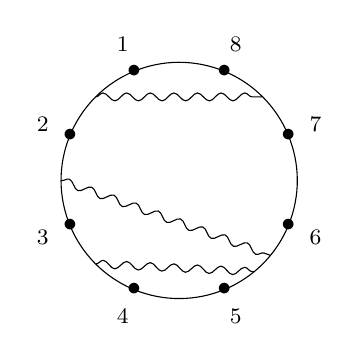
\begin{tikzpicture}[rotate=67.5,baseline=(current bounding box.east)]
	\begin{scope}
	\drawWLD{8}{1.5}
	\drawnumbers
	\drawprop{1}{0}{7}{0}
	\drawprop{3}{0}{5}{-1}
        \drawprop{2}{0}{5}{1}
		\end{scope}
	\end{tikzpicture}\eas and $W' = (\{(1,4), (3,5), (6,7), (8,1), (8,1)\}, [8])$ as \bas W'\ =\ 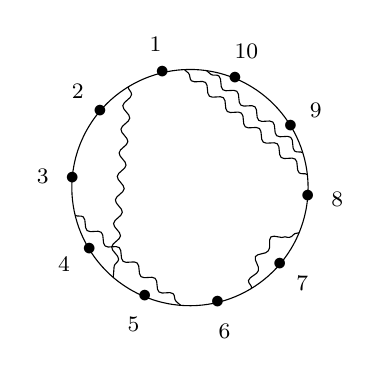
\begin{tikzpicture}[rotate=67.5,baseline=(current bounding box.east)]
	\begin{scope}
	\drawWLD{10}{1.5}
	\drawnumbers
	\drawprop{1}{0}{4}{0}
	\drawprop{3}{0}{5}{0}
        \drawpropbend{6}{0}{7}{0}{35}
	\drawprop{8}{1}{10}{-1}
 	\drawprop{8}{-2}{10}{2}
		\end{scope}
	\end{tikzpicture}\;.\eas 
Note that the pairs indicating the propagators are unorderer. That is if the propagator $p$ ends on the third and fifth edges, we may write $p = (3,5)$ or $p(5,3)$. In this paper, we use the convention that one may write $p = (i, j) = (j,i)$. That is, the two indices do not correspond to an ordered pair, or impose an orientation on $p$. Rather, they are simply the edges on which the propagators end. Furthermore, we use the convention that if two propagators have endpoints on the same edge, they are drawn so that they do not cross. 

In the diagram $W$, the propagators $p = (3,5)$ and $r = (2,5)$ both end on the the $5^{th}$  edge of the diagram. By Definition \ref{dfn:adjascentprops}, these two edges are adjascent. When we need to refer to their positioning on the $5^{th}$ edge, refer to them as $q_1 = p$ and $q_2 = r$. Consider the set of these two propagators: $Q = \{p, r\}$. Then $V_Q = \{ 2, 3, 4, 5, 6\}$. Callthe remainining propagator in the diagram $s$: $s = (1, 7)$. Then $F(s) = \{1, 7, 8\} = V_Q^c$. In particular, the vertex $2$, which supports both $s$ and $r$, and therefore isn't an element of $F(s)$.
\end{eg}


In the physics literature, we are only intersted in a certain subclass of these graphs, called admissible Wilson loop diagrams. An \emph{admissible} Wilson loop diagram, $W = (\cP, [n])$ satisfies the following conditions:
\begin{enumerate}
\item \textbf{Non-crossing} No pair of propagators $p, q \in \cP$ cross in the interior of $W$. That is, for two propagaotors $p = (i,j), \; q = (k, l) \in \cP$ written such that $i <j$ and $k <l$ in natural linear order on $[n]$, if $i < k$ then $l <j$. 
\item \textbf{Local Density} Any subset of propagators $ P \subset \cP$ is supported by at least 3 more vertices than the number of propagators in $P$: $|V_P| \geq |P| + 3$. 
\item \textbf{Global Density} There are at least 4 more vertices in the diagram than there are propagators. That is $n \geq |\cP| + 4$.
\end{enumerate} 

Note that the diagram $W$ above is admissible, while $W'$ is not. Furthermore, note that local density implies that one cannot have a propagators $p = (i, i+1)$ or pairs of propagators with the same endpoints: $p = q = (i, j)$.

For the remainder of this paper, we restrict our attention only to admissible Wilson loop diagrams. We denote by $\cW_{k,n}$ to be the set of all Wilson loop diagrams with $k$ propagators and $n$ vertices: $\cW_{k,n} = \{ (\cP,[n])| \textrm{ admissible }; \; |\cP| = k\}$. 


\subsection{Variable valued matrices and matroids \label{sec:matrices and matroids}}

Wilson loop diagrams have a natural matrix representation with real independent variable entries that bridges the combinatorics of the diagrams to matroids and to geometric subspaces of the positive Grassmannians. Before introducing this representation, we  define some notation around matrices with algebraically independent invertible variables, and recall some facts about Matroids

\begin{dfn} \label{dfn:variablevaluedmatrix}
Let $\cV = \{V_1, V_2, \dots, V_k\}$ be a collection of subsets of $\{1,2,\dots,n\}$. Let $\mathbf{x}=\{x_{i,j}\}$ be a set of algebraically independent invertible variables. Define $M_{\mathcal{V}}\in M_{k,n}$ to be the $k \times n$ matrix having $x_{i,j}$ as its $i,j$ entry if $j \in V_i$ and $0$ otherwise.
\end{dfn}

One can realize a matrix $M_\cV$ at a point $\mathbf{x}=\{x_{i,j}\} \in \R^{|\mathbf{x}|}$ to get a real valued matrix. We can vary the points in $\R^{|\mathbf{x}|}$ to parametrize a family of real valued $k \times n$ matrices. Furthermore, by ignoring any such matrices of less than full rank, we may parametrize a subset of $\Grall(k,n)$.

Let $M^{\rk k}_{k,n}$ be the set of $k \times n$ matrices of full rank. Then the standard quotient map takes $M^{\rk k}_{k,n}$ to $\Grall(k,n)$ \ba \phi: M^{\rk k}_{k,n} \rightarrow \Grall(k,n)  \label{eq:maps}\ea

\begin{dfn} \label{dfn:loci}
  Let $L(\cV)$ is the set of point of $\Grall(k,n)$ that can be realized by setting the entries of $M_\cV$ to real values. In other words, $L(\cV) = \phi (M_{\cV} \cap M^{\rk k}_{k,n})$.  
\end{dfn}

Finally, sometimes, we need to refer to the subsets in $\cV$ that intersect a subset  $S \in \{1,2,\dots,n\}$. These sets correspond to the rows of $M_{\cV}$ have non-zero entries in the columns indicated by $S$. 

\begin{dfn}\label{dfn:columns}
For $S \in \{1,2,\dots,n\}$, write $\cV_S =\{V_i \in \cV |  V_i \cap S \neq \emptyset\}$. 
\end{dfn}

Matrices of the form $M_\cV$ define matroids\footnote{Specifically, the class of matroids defined in this way are transversal matroids \cite{????}, as discussed in \cite{basisshapeloci}, but that is beyond the scope of this discussion.}. The remainder of this section gives a brief overview of matroids, which the expert reader may skip. 

A matroid can be defined as a set, and a set of independence conditions on said set. For instance, one can define $M = (E, \mathcal{B})$, where $\mathcal{B}$, called a basis set, is a non-empty set of subsets of $E$, each of the same size, satisfying the basis exchange condition: \bas \textrm{for  all } A \textrm{ and } B \in \cB, \textrm{ if }  a \in A\setminus B \textrm{ then } \exists b \in B \setminus A \textrm{ and } (A \setminus a) \cup b \in  \cB \;.\eas Each element of $\mathcal{B}$ is a basis of $M$ and denotes a maximal independent set. The rank of the matroid, denoted $\rk(M)$ is the unique size of all the basis sets. We may also refer to the rank of a subset of $E$, $S \subset E$. We write the rank of $S$ as $\rk(S) = \max \{|B \cap S| : B \in \mathcal{B} \}$.%, which, by abuse of notation, we also denote $\rk(S)$. The restriction of $M$ to $S$ is $M|S = \{B \cap S : B \in \calB, |B \cap S| \rk(S)\}$.

Equivalently, one can define $M = (E, \mathcal{F})$, where $\mathcal{F} = \{ F \subset E| \forall x \in E \setminus F, \rk(F \cup x) > \rk(F)\}$ is the set of flats of $M$. For any subset $S \subset E$, we can define the closure of the set $\textrm{cl}(S)  = \{x \in E | \rk(S) = \rk(S \cup x)\}$ as the smallest flat containing $S$. Note that if $S$ and $T$ are two flats, then $S \cap T$ is also a flat. 

Also equivalently, we may write $M = (E, \mathcal{C})$ where $\mathcal{C} = \{C \subset E | \forall S \subsetneq C, \; S \subset B \textrm{ for some } B \in \mathcal{B}\}$ is the set of circuits of $M$. The circuits are the minimal dependent sets, i.e. each proper subset of $C$ is independent. If $C$ and $D$ are both circuits, then $C \cup D$ is a cycle. 

Given a matroid $M = (E, \mathcal{B})$, and a subset $S \subset E$, the restriction $M|S = (S, \mathcal{B|S} = \{B\cap S| B \subset \mathcal{B} \textrm{ such that } |B \cap S| = \rk(S) \}$. The contraction is defined $M/S = (E \setminus S, \mathcal{B/S} = \{B\setminus S| B \subset \mathcal{B} \textrm{ such that } |B \cap S| \textrm{ maximal}\}$. A matroid is disconnected if it can be written as the direct sum of two matroids: $M = (E_1, \mathcal{B}_1) \oplus (E_2, \mathcal{B}_2)  = (E_1 \cup E_2 , \mathcal{B}_1 \times \mathcal{B}_2)$. Otherwise, it is connected.

A matroid is representable if it can be written as a matrix with the same independence data. In particular, since the matrices $M_\cV$ have algebraically independent non-zero entries, it is straight forward to read off the matriod assoiciated to the collection of sets $\cV$.

\begin{eg}\label{eg:variablevaluesasmatroids} \sanote{Cam: check this. I've changed this back into dependent set notation.}
Given a collection of subsets $\cV$ as in Definition \ref{dfn:variablevaluedmatrix}, we may define a matroid with a ground set consisting of the columns of $M_\cV$. That is, $E = \{1, \ldots , n\}$. Then, for each subset $S \subset E$ and corresponding set of subsets $\cV_S$ as defined in Definition \ref{dfn:columns}, the set $S$ is a circut in the matroid defined by $M_\cV$, if $\cV_S$ contains strictly fewer elements than $S$, i.e. $|\cV_S| < |S|$. More informally, since the elements of $V$ correspond to rows of $M_\cV$, and the elements of $S$ its columns, this is simply saying that the set of columns $S$ contains minimally dependent set if there are fewer rows with non-zero entries than columns indicated by $S$.  %A $k$ element subset $S \subset E$ is a basis if and only if the $k \times k$ minor corresponding to $S$, with determinants computed in the ring $\mathbb{R}(\mathbf{x})$, is \hlfix{nonzero.}{i switched this definition to be in terms of bases. commented out, it was inaccurate but in terms of independent sets. if we want the independent set version, i can add that.} %
\end{eg}

\begin{dfn}\label{dfn:matroid}
We write $M(\cV)$ to denote the matroid defined by the variable valued matrix $M_\cV$. 
\end{dfn}



A positroid is a matroid, endowed with a cyclic ordering on the ground set, that can be realized as a matrix with all positive minors. Note that if $M$ is a positroid, as a matroid it is invariant under any cyclic permutation of the ground set. However, as a postroid, in order to  preserve the nonnegativity of the minors, it is only invariant under cycic permutations of the ground set. Let $<_a$ denote the $a$-th cyclic shift of the standard order on $\{1, \dots, n\}$. So, $a <_a (a+1) <_a \cdots <_a (a-1)$. These cyclic orderings on $E$ define Gale orderings on the subsets, $\{s_1 <_a s_2 <_a \cdots <_a s_k\} \leq_a \{t_1 <_a t_2 <_a \cdots <_a t_k\}$ if and only if $s_i \leq_a t_i$ for all $1 \leq i \leq k$. The collection of minimal basis sets for each cyclic shift of the Gale ordering gives the Grassmann necklace associated to a positroid. See \cite[Chp ??]{Postnikov} for the original construction or \cite{non-crossingpartiion} for a good exposition.

One way to determine if a matroid is a positroid is to look at its flacets. A flacet, $F$, of a (connected) matroid $M$ is any subset of $M$ such that $M|F$ and $M/F$ are both connected. If $M$ is a positroid, then every flacet is a cyclic interval of the ground set. Furthermore, for any matroid, any flacet is a cyclic flat.

Positroid varieties define subsets of $\Grall(k,n)$ that give a CW complex when restricted to $\Gr(k,n)$ \cite[Chapter ]{Postnikov}. We refer to the positroid cells by the letter $\Sigma$.

\begin{dfn}If the matroid $M(\cV)$, is a positroid, let $\Sigma(\cV)$ and $\overline{\Sigma(\cV)}$ be associated open and closed positroid varieties respectively. As such, it defines a subspace of $\Grall(k,n)$. We write $\Sigmapos(\cV) = \Sigma(\cV) \cap \Gr(k,n)$ and $\overline{\Sigmapos(\cV)} = \Sigma(\cV) \cap \Gr(k,n)$ to be the open and closed positroid cells defined by restricting to $\Gr(k,n)$. \end{dfn} 

In this way, the word positroid has both a geometric meaning (as a subset of a Grasmannian) and a matroidal meaning (as a matroid where every flacet is a cyclic flat). These two meanings are tightly related in that every geometric positroid can be represented matroidally as a positroid and vice versa. It should be clear from context whether the word positroid is referring to a combinatorial object or a subset of the Grassmannian. %When we refer to the matroid of a point in the positive Grassmanian, we refer to the positroid of that point in the matroidal sense. When we say the positroid of a matrix, we refer to the geometric meaning.

Similarly, we write $\Lpos(\cV)$ to be the restriction of $L(\cV)$ to $\Gr(k,n)$. Note that while the geometrically motivated subspaces of $\Grall(k,n)$, $\Sigma(\cV)$, are in one to one correpondence with the subspaces defined by matrices, $L(\cV)$, these two subspaces are not the same.

We conclude this section with an example of how $L(\cV)$, $\Sigma(\cV)$, and $\overline{\Sigma(\cV)}$ differ.

\begin{eg} \label{eg:closuresmatch}
This example illustrates the differences between the sets $L(\cV)$, $\Sigma(\cV)$, and $\overline{\Sigma(\cV)}$. Let
\bas M_{\cV} =
\begin{bmatrix}
x_{p,1} & x_{p,2} & 0 &x_{p,4} & x_{p,5} & 0 \\
x_{q,1} & x_{q,2} & 0 & 0 & x_{q,5} & x_{q,6}
\end{bmatrix}\eas  Note that this matrix corresponds to a Wilson loop diagram, but the result demonstrated in this example is much more general. Let $\Sigma(\cV)$ and $\overline{\Sigma(\cV)}$ be the associated open and closed positroid cells respectively.

The point represented by
\begin{displaymath}
\begin{bmatrix}
1 & 1 & 0 & 1 & 1 & 0 \\
1 & 1 & 0 & 0 & 1 & 1
\end{bmatrix}
\end{displaymath}
\noindent
is in $L(\cV) \setminus \Sigma(\cV)$, since the minor $ \Delta_{12}$ vanishes. \hlfix{}{part of the example was talking about R(V), which hadn't been defined yet. i commented it out, but should possibly include that part of the example later.}%Hence,
%%
%\begin{displaymath}
%R(\cV) = (x_{p,1}x_{q,2} - x_{p,2}x_{q,1}) x_{p,1} x_{p,4} x_{p,5} x_{q,2} x_{q,5} x_{q,6}
%\end{displaymath}
%\noindent
%vanishes at this point.

The point represented by
\begin{displaymath}
\begin{bmatrix}
1 & 0 & 0 & 1 & 0 & 1 \\
0 & 1 & 0 & 1 & 1 & 1
\end{bmatrix}
\end{displaymath}
\noindent
is in $\Sigma(\cV) \setminus L(\cV)$ since there is no point in $L(\cV)$ where $\Delta_{45},\Delta_{56} \neq 0$ and $\Delta_{46} = 0$.

The point represented by
\begin{displaymath}
\begin{bmatrix}
0 & 0 & 0 & 0 & 1 & 0 \\
0 & 0 & 0 & 1 & 0 & 1
\end{bmatrix}
\end{displaymath}
\noindent
is in $\overline{\Sigma(\cV)} \setminus (\Sigma(\cV) \cup L(\cV))$.
\end{eg}




\section{Geometry of Wilson loop diagrams \label{sec:WLDgeom}}

We are now ready to apply the notation above to Wilson loop diagrams. We first show that a Wilson loop diagram can be associated to a matrix with real independent variable entries, and thus to a matroid. The authors of \cite{wilsonloops} show that these matroids are infact all positroids, $\Sigma(\VP)$. Then we define the integrals associated to each Wilson loop diagram, and show that the poles of the integrand appear on the boundary of $\Sigmapos(\VP)$. 

\subsection{Wilson loop diagrams as positroids \label{sec:WLDmatroid}}

In order to associate a matrix to a Wilson loop diagram, $W = (\cP, [n])$,  to each propagator $p \subset \cP$ associate a $4$ dimensional subspace of $\RP^{n+1}$ of the form \bas Y_p = \begin{cases}  x_{p,i} &  i = 0 \textrm{ or } i \in V_p \\ 0 &  \textrm{else,}\end{cases} \eas where $x_{p,i}$ are algebraically independent real valued variables \cite{a physics paper}.Then one may associated to $W$ a subspace of $\Grall(k, n+1)$ given by the linear span of the $Y_p$. 

In other words, for each Wilson loop diagram $(\cP, [n])$, we have two sets of subsets \bas \YP = \{ V_p \cup 0 | p \in \cP\} \quad \textrm{ and } \quad \VP = \{ V_p | p \in \cP\} \eas  that define two matrices $M_{\VP}$ and $M_{\YP}$. These define subspaces of $\Grall(k, n+1)$ and $\Grall(k, n)$ respectively, that we call $L(\YP)$ and $L(\VP)$ as in Definition \ref{dfn:loci}.

\begin{eg} \label{eg:matrices}That is, given the Wilson loop diagram $W$ in example \ref{eg:admissible}, with $p = (3,5)$, $r = (2,5)$, and $s = (1,7)$ one may write \bas M_{\YP} = \begin{bmatrix}  x_{p,0} & 0 & 0 &x_{p,3} & x_{p,4} &  x_{p,5} & x_{q,6} & 0 & 0 \\ x_{r,0} & 0 & x_{r,2} & x_{r,3} & 0  &x_{r,5} & x_{r,6} & 0 &0 \\ x_{s,0} & x_{s,1} & x_{s,2} & 0 &0 &0 &0 &x_{s,7} & x_{s,8} \end{bmatrix} \;.\eas

We define the matrix $M_{\VP}$ to be the one defined by ignoring the first column of $M_{\YP}$.  In the running example, \bas M_{\VP} = \begin{bmatrix}  0 & 0 &x_{p,3} & x_{p,4} &  x_{p,5} & x_{q,6} & 0 & 0 \\ 0 & x_{r,2} & x_{r,3} & 0  &x_{r,5} & x_{r,6} & 0 &0 \\  x_{s,1} & x_{s,2} & 0 &0 &0 &0 &x_{s,7} & x_{s,8} \end{bmatrix} \;.\eas
\end{eg}

 
\begin{rmk}
Note that, as a subspace of $\Grall(k, n)$ (resp. $\Grall(k, n+1)$), or ordering of the rows in $M_{\VP}$, resp. $M_{\YP}$ do not matter.
\end{rmk}

\begin{rmk}
It is also worth noting that in previous literature, the matrices $M_{\YP}$ and $M_{\VP}$ were denoted $C_*(W)$ and $C(W)$ respectively. However, in this paper, we wish to exploit the results of \cite{basisshapeloci} to understand the properties of the parametrized spaces, and therefore, change the naming conventions. 
\end{rmk}

Note that in this setup, for $W = (\cP, [n])$ and $V \subset [n]$, the set $\Prop(V)$ indicates the rows of $M_{\VP}$ that have non-zero entries in the collumns indicated by $V$. That is, in the notation of Defintion \ref{dfn:columns}, $\Prop(V) = \VP_V$. 

The matroidal properties of Wilson loop diagrams derived in \cite{Wilsonloops}  can be verified by considering the independent columns of $M_{\VP}$.
\begin{enumerate} 
\item Theorem [3.9] of \cite{wilsonloops} states that a set of vertices of a Wilson loop diagram, $(\cP, [n])$  is independent if and only if no subset supports fewer propagators than vertices in the subset. I.e. $V \subset [n]$ is independent if, for all $U \subseteq V$, $\Prop(U) \geq |U|$. In terms of rows and columns of $M_{\VP}$, this simply states that any set of columns of $M_{\VP}$ contains a dependent subset if said subset is non-zero on fewer rows than columns in the subset, which is consistent with the cycle condition laid out in Example \ref{eg:variablevaluesasmatroids}
\item Corrollary \cite[3.39]{wilsonloops} shows that all admissible Wilson loop diagrams, in particular those satisfying the non-crossing and local density conditions, correspond to positroids. This means that, as matroids, the Wilson loop diagrams can be represented by matrices with all positive maximal minors. That is, the subspace of $\Grall(k,n)$ parametrized by $M_{\VP}$ intersects $\Gr(k,n)$.
\end{enumerate}

\begin{eg}\label{eg:wldmatroid} For instance, in $W$  from Example \ref{eg:admissible}, the vertices $\{7,8\}$ are a cycle since they only support one propagator between them. In fact, the define a circuit. On the other hand, the vertices $\{3,4\}$ support two propagators, and thus are independent. Consider the set of proppagators $P = \{ (2, 5), (3, 5)\}$. Then $F(P) = \{ 1, 7, 8\}$. This is a flat of rank $2$. In \cite{wilsonloops}, set of the form $F(P)$ are called propagator flats, and the author shows that the cyclic flats of the matroid assoicated to $W$ are propagator flats.
\end{eg}

Furthermore, work of \cite{basisshapeloci} gives insight into the geometry of Wilson loop diagrams in $\Gr(k,n)$. In \cite[Theorem 8.4]{basisshapeloci} the author shows that for a Wilson Loop diagram $W = (\cP, [n])$, the closure of the locus, $L(\VP)$, corresponds to the closure of the positroid: $\overline{L(\VP)} = \overline{\Sigma(\VP)}$, \sanote{changed this to be over the full Grassmannian. Correct?} and thus, in the positive Grassmannians as well, the subspace parametrized by the matrices $M_{\VP}$ corresponds to a positroid cell, up to a space of measure 0, $\overline{\Lpos(\VP)} = \overline{\Sigmapos(\VP)}$, as illustrated in Example \ref{eg:closuresmatch}.

The author of \cite{basisshapeloci} also shows each $\Sigma(\VP)$ is a $3k$ dimensional space. More generally, the author shows, using slightly different notation:

\begin{thm}[Theorem 3.2, \cite{basisshapeloci}]\label{res:minimalrep}
Given a variable valued $k \times n$ matrix $M_\cV$ with $m$ non-zero entries representing a positroid  $\Sigma(\cV)$, the following are equivalent:
\begin{enumerate}
\item $\dim(\Sigma(\cV)) = m -k$ 
\item $M_\cV$ has the smallest number of non-zero variable entries of any variable valued matries representing $\Sigma(\cV)$
\item For all $\mathcal{T} \subseteq \cV$, \bas |\bigcup_{T \in \mathcal{T}}T| \geq \max_{T \in  \mathcal{T}} (|T|) + |\mathcal{T}| -1 \;. \eas
\end{enumerate}
\end{thm}


In \cite[section 2.3]{non-orientable}, the authors show that  the subspace of $\Grall(k,n)$ parameterized by $M_{\YP}$, can be viewed as a real $k$ vector bundle over the space parametrized by $M_{\VP}$, i.e.  $\cup_{W \in \cW_{k,n}}L(\YP) \rightarrow \cup_{W \in \cW_{k,n}}L(\VP)$. Restricting to any given Wilson loop diagram gives a trivial vector bundle $L(\YP) \rightarrow L(\VP)$. As shown in Theorem 2.29 of loc. cit., the space $\cup_{(\cP, [n]) \in \cW_{k,n}}L(\YP)$ need not be orientable. 


\subsection{Integrals and poles \label{sec:integrals}}

The goal of this paper is to show that the spurious poles of the integrals associated to Wilson loop diagrams cancel in the calculation of the full amplitude. In this section we define the integrals and show that the poles lie on the boundary of the associated positroid cell ($\Sigmapos(\VP)$).

Recall that there are two types of singularities to this theory: the physical poles and the spurious poles. The physical poles arise when the vectors representing the particles do not span $\R^4$, as one expects in a physical theory with infrared singularites. The sprurious poles are those that arise in each summand of the integrals involved in calculating the three level scattering amplitude. These should cancel in the sum. In this section, we discuss the algebraic and geometric properties  of these poles. 

\subsubsection{Integrals associated to Wilson loop diagrams}
The Wilson loop diagrams represent the tree level contributions to the scattering amplitudes in the physical theory N=4 SYM. The holomorphic Wilson loop for $n$ particles and $k$ propagators gives the contribution to the n particle scattering amplitude of N=4 SYM by $k$ propagators. The tree level contribution to this amplitude is given by a sum of integrals associated to admissible Wilson loop diagrams: \ba \cA_{k,n}^{tree} = \sum_{(\cP, [n]) \subset \cW_{k,n}} I(\VP) \;.\label{eq:treelevelamplitude}\ea The scattering amplitude is a functional on the particles of the theory, represented in twistor space. In this case, the external data are represented as $n$ sections of a $k$ dimensional real vector bundle over a real twistor space, $\{Z_1, \ldots, Z_n\}$  such that the $n \times n+4$ matrix who's $i^{th}$ row is $Z_i$ has positive maximal minors. Furthemore, we fix a guage section, $Z_0$, which can be taken, without loss of generality to be a $0$ section. We define the matrices \bas \cZ = \begin{bmatrix} - & Z_1& - \\ & \vdots &  \\ - & Z_n& -\end{bmatrix} \; ; \; \cZ_* = \begin{bmatrix}- & Z_0& - \\  - & Z_1& - \\ & \vdots & \\  - & Z_n& -\end{bmatrix} \; .\eas Note from above, the matrix $\cZ$ has positive maximal minors, while the matrix $\cZ_*$ may not.

Before we define the actual integral, $\cI(\VP)$, recall that if multiple propagators end on the $e^{th}$ edge, we order them according to their proximity to the vertex $e$. We are now ready to define the integrals assoicated to each Wilson loop diagram $W = (\cP, [n])$, with $k = |\cP|$:

\begin{dfn} \label{dfn:I(W)} \bas \cI(\VP) (\cZ_*)  = \int_{(\RP^4)^k} \frac{\prod_{p \in \cP} \prod_{v \in V_p} dx_{p, v}}{R(\VP)} \delta^{4k|4k}(M_{\YP} \cdot \cZ_*) \eas where, for $X$ a $k \times k+4$ matrix, \bas \delta^{4k|4k}(X) = \prod_{b =1}^k (X_{b, 4+b})^4\delta^4((X_{b,1},X_{b,2},X_{b,3},X_{b,4}))  \eas and $R(\VP)$ is a polynomial determined from the $W$ as follows: 
\begin{enumerate}
\item Define $R_e = x_{q_1, e+1} \big(\prod_{r = 1}^{s-1} (x_{q_r, e}x_{q_{r+1}, e+1} - x_{q_r, e+1}x_{q_{r+1}, e})\big) x_{q_s, e}$
\item $R(\VP) = \prod_{e \in [n]} R_e$
\end{enumerate} \end{dfn}

Appendix \ref{sec:appendix} gives examples and context for calculations done with these integrals. 

There are a few features to note in this defintion. First, notice that the spurious poles of the theory correspond to setting the factors of $R(\VP)$ to zero. Specifically, by equations \eqref{eq:matrixvalues} in Appendix \ref{sec:appendix}, the variables $x_{p,0}$ localize to $0$ when the vectors representing the particles do not span $\R^4$. This corresponds to the physical poles of the theory. The spurious poles occur when  $x_{p,0} \neq 0$, but the polynomial $R(\VP)$ goes to $0$. See \cite{casestudy, HeslopSteward, AmplituhedonSquared} for more calculations of this form. 

Secondly, note that in this definition, we take the integral over $(\RP^4)^k$. In particular, the polynomial $R(\VP)$ is defined over $(\RP^4)^k$, and not over $L(\VP)$. Note that by a toric action, we may consider $M_{\YP}$ as a subspace of $(\RP^n)^k$, and since each row has exactly five non-zero entries, we may view each Wilson loop diagram as an isomorphism from $(\RP^4)^k$ to $M_{\YP}$. Finally, by the map in equation \eqref{eq:maps}, we may study the vanishing locus of $R(\VP)$ as a subspace of $L(\YP)$. \sanote{Changed this significantly}


Thirdly, in \cite{wilsonloops}, the authors show that the matroid $M(\VP)$ is a positroid, i.e. it $L(\VP)$ intersects the non-negative Grassmannian. Due to the parallels with the Amplituhedon, we are interested in the non-negative geometry of the spaces defined by the Wilson loop diagrams. In \cite{basisshapeloci}, the author shows that \ba \overline{\Lpos(\VP)} = \overline{\Sigmapos(\VP)} \label{eq:density}\;.\ea  In other words, up to a space of measure $0$, the non-negative space parametrized by the Wilson loop diagrams, $\{V_p\} \subset (\RP^{n})^k$ and $M_{\VP} \subset (\R^{n \times k})$ also parametrize positroid cells in the positive Grassmannians. 

Finally, returning to the main purpose of this paper, we wish to show that  the poles of these integrals (corresponding to spurious poles) cancel in the tree level amplitude. Equation \eqref{eq:treelevelamplitude} shows that $N^kMHV$ (tree level) amplitude on $n$ points is given by the sum of all the $I(\VP)$, for $(\cP, [n]) \in \cW_{k,n}$. Theorem \ref{res:polesonboundaries} shows that the spurious poles all fall on the boundaries of a geometric space defined by these diagrams. Then Theorem \ref{res:deg1polescancel} we show that the poles that fall on codimension 1 boundaries cancel.

However, unlike in the Amplituhedron story, one cannot assoiciate a geometric meaning to the sum of these integrals. In \cite{non-orientable}, the authors show that while each subspace $\Lpos(\YP)$ is orientable, the union of said spaces are not. Therefore, one cannot interpret the sum of the associated integrals as the volume of a geometric space. This result has also been shown explicitly and separately in \cite{HeslopStewart} which explicitly calculates a contradiction that occurs if one attempts this interpretation.

Here, we propose a different geometric interpretation of the sum of these integrals. The space $\Lpos(\YP)$ forms a $k$ vector bundle over $\Lpos(\VP)$ \cite{non-orientable}: $\Lpos(\YP) \rightarrow \Lpos(\VP)$. One can consider $\overline{\Lpos(\YP)}$ as the closure of a $k$-dimensional line bundle over $\overline{\Lpos(\VP)}$ \cite{non-orientable}. Then, we may consider the cancelation of spurious poles on any section of the bundle, i.e. after fixing values to the variables $x_{p, 0}$. In fact, for the spurious poles, one typically sets the values of $x_{p,0}$ to be $\pm 1$, and factors of $R(\VP)$ evaluates to $0$ \cite{??}. The physical poles of the tree level amplitude $A_{k,n}$ arise when the variables $x_{p, 0} = 0$. 


\subsubsection{Geometry of spurious poles}

In this section, we investigate the geometry of the spurious poles of the Wilson loop diagrams, or the factors of the polynomial $R(\VP)$. We give three results showing that these factors are closely related to the geometry underlying the positroid $\Sigma(\VP)$. In fact, the polynomial is exactly the product of the square free factors of the minors identified in the Grassmann Neckace of $\Sigma(\VP)$. The zero loci of the factors of $R(\VP)$ lie on the the boundary of $\Sigma(\VP)$ and the codimension one zero loci are dense in the codimension one boundaries of $\Sigma(\VP)$. 

In \cite{GWLDCII}, the authors show that the prime factors of $R(\VP)$ to are also the prime factors of the product of the minors defined by the Grassmann necklace of $\Sigma(\VP)$. We restate it here using the notation of this paper.

Recall that the matrix $M_{\cV}$ is parametrized by the independent variables $\bf{x}$, with one algebraically independent variable in each non-zero entry.

\begin{thm} \cite[Proposition 5.3]{GWLDCII} \label{res:prop alg gives rad}
Write $\cI = \{I_1, \ldots I_n\}$ be the Grassmann necklace assoicates to the positroid cell $\Sigma(\VP)$. Let $\Delta_{I_i}(\bf{x})$ be polynomial in $\bf{x}$ defined by the minor of $M_{\VP}$ indicated by the columns indexed by $I_i$.  Then \begin{enumerate}
 
   \item Each $\Delta_{I_i}(\bf{x})$ splits into linear and quadratic factors.  All linear factors of  $\Delta_{I_i}(\bf{x})$ are single variables and all irreducible quadratic factors are $2\times 2$ determinants of single variables.
    \item Quadratic factors in $\Delta_{I_i}(\bf{x})$ arise precisely when propagators $p$ and $q$ are supported on a common edge $a$.
    \item The factor $r_e$ divides $\Delta_{I_e}(\bf{x})$.
    \item The ideal generated by $R(\VP)$ is the radical of the ideal generated by $\prod_{i=1}^{n}\Delta_{I_i}(\bf{x})$.
  \end{enumerate}
\end{thm}

We can generalize this result to define a polynomial given by a minimal parametrization of a positroid cell. 

\begin{dfn}\label{dfn:RV}
Let the set of subsets $\cV$ define a matroid $M(\cV)$. If $M(\cV)$ is also a positroid, let $\cI =  \{I_1, \ldots I_n\}$ be the associated Grassman Necklace. Then define $R(\cV)$ to be the polynomial formed by the product of the prime factors of $\prod_{i=1}^{n}\Delta_{I_i}(\bf{x})$ in the variables $\{x_{i,j}\}$ defined by the set $\cV$. That is, $R(\cV) = \textrm{rad}(\prod_{i=1}^{n}\Delta_{I_i})(\bf{x})$. 
\end{dfn}

We note that here, $R(\cV)$ is a polynomial in the matrix entries $x_{p,i}$. The radicals taken are over the polynomial ring $\R[\bf{x}]$, defining a variety in the space of $n \times k$ matrices. To pass to the Grassmannian and obtain the variety $\overline{\Sigma(\cV)}$, one must consider the image under the map in \eqref{eq:maps}. 

In particular, there may be multiple polynomials arising from the same Grassmann Necklace defining the positroid variety $\Sigma(\cV)$, as illustrated in the following example.

\begin{eg} \label{eg:differentpolys} Note that the polynomial $R(\cV)$ is dependent on the minimal parametrization of the postroid defined by the Grassmann Neclace $\cI$.  For instance, in \cite{GWLDCI}, the authors give conditions for when multiple Wilson loop diagrams can correspond to the same positroid cell. For example, the $2 \times 6$ matrices defined by $\cV_1 = \{\{1, 2, 4, 5\}, \; \{1, 2, 3, 4\} \}$ and $\cV_2 = \{\{1, 2, 4, 5\}, \; \{2, 3, 4, 5\} \}$ both correspond to the positroid variety with Grassmann Necklace $\cI = \{12, 23, 34, 45, 51, 12\}$. However \bas R(\cV_1) = x_{1,2}(x_{1,1}x_{2,2}- x_{2,1}x_{1,2})x_{2,1}x_{2, 3}x_{2,4}x_{1,4}x_{1,5}  \quad \textrm{while} \\ R(\cV_2) =  x_{1,1}x_{1,2}x_{2,2}x_{2, 3} x_{2,5}(x_{1,4}x_{2,5}- x_{2,4}x_{1,5})x_{1,4}\;.\eas Both correspond to the polynomial formed by the product of the prime factors of $\prod_{i=1}^{n}\Delta_{I_i}(\bf{x})$ under the corresponding coordinate system.

This is different from the approach elsewhere in the literature, eg \cite{GalashinLam, SSBW}, where similar polynomials are defined on the Pl\"{u}cker coordinates.

\end{eg}

Next, we to show that the factors of $R(\VP)$ vanish on the boundary of the associated positroids. This has been shown explicitly in the case of $n = 6$ and $k=2$ \cite{casestudy}, however, has not been shown in general.


\begin{prop}\label{res:vanishonbdny} 
If the matrioid $M(\cV)$ is also a positroid, then the factors of $R(\cV)$ vanish on the boundary of the positroid variety $\Sigma(\cV)$.
\end{prop}


\begin{proof}
Let $GN(\cV) = \{I_1, I_2, \dots, I_k\}$ be the Grassmann necklace associated $\Sigma(\cV)$. From Definition \ref{dfn:RV}, 
%
\begin{displaymath}
R(\cV) = \mathrm{rad}\left(\prod_{i = 1}^{k} \Delta_{I_i}(\bf{x})\right).
\end{displaymath}
%
From Theorem 5.15 in \cite{knutsonlamspeyerjuggling}, the ideal of functions defining the variety $\overline{\Sigma(\cV)}$ is generated by $\{\Delta_I | I_b \not \leq_b I; \; b \in I\}$ \st{$\{\Delta_I : I \notin M_{\cV}\}$} where $\leq_b$ indicates the Gale ordering.\todo{Cam: is this correct?} From in \cite[Theorem 5.1]{basisshapeloci}, $L(\cV) \subset \overline{\Sigma(\cV)}$ and hence every function vanishing on $\Sigma(\cV)$ vanishes on $L(\cV)$. Theorem 5.1 in \cite{knutsonlamspeyerjuggling} implies that the open positroid variety $\Sigma(\cV)$ is defined as a subset of $\overline{\Sigma(\cV)}$ by requiring certain minors to be non-vanishing. Namely, 
%
\begin{displaymath}
\Delta_{I_1}, \Delta_{I_2}, \dots, \Delta_{I_k} \neq 0.
\end{displaymath}
%
We may consider the minors $\Delta_{I_i}$ either as Pl\"{u}cker coordinates, or as polynomials in variables defining $M_{\cV}$. Using the latter interpretation, we note that the polynomial $R(\cV)$ vansihes exactly where at least one of the $\Delta_{I_i}(\bf{x})$ vanish, ie exactly  of $L(\cV)$ defined 
%
\begin{displaymath}
L(\cV) \setminus \Sigma(\cV) \subset \overline{\Sigma(\cV)} \setminus \Sigma(\cV). \qedhere
\end{displaymath}
\end{proof}

We can use Proposition \ref{res:vanishonbdny} to show that for Wilson loop diagrams, factors of $R(\VP)$ that vanish on codimension 1 boundaries of $\Sigma(\VP)$ have a locus that is dense in the corresponding positroid. \sanote{Cam, did I break this?}



\begin{thm}\label{res:polesonboundaries}
Let $W=(\mathcal{P},[n])$ be an admissible Wilson loop diagram and let $L' \subset L(\VP)$ be the vanishing locus of a single factor of $R(\VP)$ inside $L(\VP)$ and suppose that $L'$ has codimension $1$ in $L(\VP)$. Then, \hlfix{$\overline{L'\cap \Gr(k, n)} = \overline{\Sigma'}$, where $\Sigma'$ is a positroid cell}{do we need to restrict to the positive grassmanninans here?} in the boundary of $\Sigmapos$. \end{thm}



\begin{proof}
From Theorem \ref{res:prop alg gives rad}, $R(\VP)$ is the product of individual entries and two by two minors of $M_{\VP}$. Suppose first that $L'$ is a codimension $1$ locus obtained by setting a single variable $x_{p,i}$ to zero. Then, $L'$ is the subset of the Grassmannian consisting of row spaces of matrices of the form $M_{\VP}$ where $x_{p,i}$ is set to zero and all other entries are evaluated at real numbers. \hlfix{Theorem CITE THEOREM  implies that a generic point in $L'$ represents the same matroid.}{Same matroid as what? as another generic point? should this be moved up in the paper?} Since the positroid stratification is coarser than the matroid stratification, \hlfix{a generic point in $L'$ is contained in the closure of some positroid $\Sigma' \subset \overline{\Sigma}$}{???}. Proposition \ref{res:vanishonbdny} implies that $L' \subset \overline{\Sigma} \setminus \Sigma$ and so $\Sigma' \neq \Sigma$. Since $L'$ was assumed to be codimension $1$, the matroid represented by a generic point in $L'$ is in fact $\Sigma'$. Then, Theorem CITE THEOREM implies that $\overline{L'} = \overline{\Sigma'}$, as desired.

Next, suppose that $L'$ is a codimension $1$ boundary obtained by setting a two by two minor of $M_{\mathcal{P}}(\mathbf{x})$ to zero. As in Lemma \ref{lem:simplifyR(W)}, $L'$ may be represented by reparameterizing this two by two minor in $M_{\VP}$, then setting one of the new parameters to zero. Let $M'$ denote the variable valued matrix obtained by this change of variables. Generic points in $L'$ represent the same matroid, namely the matroid whose bases are the minors $M'$ which aren't identically zero. Proposition \ref{res:vanishonbdny} implies $L' \subset \overline{\Sigma} \setminus \Sigma$. Then, since $L'$ has codimension $1$ in $\overline{\Sigma}$, the matroid represented by a generic point in $L'$ is a positroid $\Sigma'$. The open positroid $\Sigma'$ has a parameterization via a Marsh-Reitsch matrix $R$ in the same number of variables as $M'$. Then, as in the proof of CITE THEOREM, $M'$ and $R$ are generically related by a change of basis matrix and thus $\overline{L'} = \overline{\Sigma'}$.
\end{proof}

\begin{eg} \label{eg:codim2}
Note that not all factors of $R(\VP)$ correspond to codimension 1 subspaces of $\Sigma(\VP)$. 

For instance, consider the diagram in Example \ref{eg:closuresmatch}. Setting $x_{p,4}$ to $0$ gives the matrix \bas M' =
\begin{bmatrix}
x_{p,1} & x_{p,2} & 0 &0 & x_{p,5} & 0 \\
x_{q,1} & x_{q,2} & 0 & 0 & x_{q,5} & x_{q,6}
\end{bmatrix}, \eas which can be written as $M_{\cV}$ with $\cV = \{V_1 = \{ 1, 2, 5\}, V_2 = \{1, 2, 5, 6\}\}$. Note that while $ |\bigcup_{V \in \cV}V|  = 4$,
\begin{displaymath}
\max_{V \in  \cV (|V|)} + |\cV| -1  = 4 + 2 - 1.
\end{displaymath}
Therefore the third equivalent statement of Theorem \ref{res:minimalrep} does not hold, and thus $M_{\cV}$ is not parametrize a $5$ dimensional subspace of $\Grall(k,n)$. Since, by display (1) of \cite{basisshapeloci}, $5$ was an upper bound on the dimension of $L(\cV)$, setting $x_{p,4}$ must correspond to a higher codimension subspace of $\Sigma(\VP)$. In fact, direct calculation shows that this factor lies on a codimension 2 locus.

\end{eg}

We show in section \ref{sec:boundarysanspoles} that the converse of Theorem \ref{res:polesonboundaries} does not hold. Namely, not every co-dimension one boundary of $\Sigma(\VP)$ contains the vanishing loci of a factor of $R(\VP)$. 


\subsection{Cluster algebras, frozen variables, Grassmann Necklaces \label{sec:clusteralgebras}}

We conclude this section with a brief aside, noting that the polynomial $\prod_{I_i \in \cI}I_i$ has appeared in relation to a cluster algebra associated to the positroid $\Sigma(\cV)$ where $\mathcal{I} = \{I_1,I_2, \dots, I_k\}$ be the Grassmann necklace associated to $\Sigma(\cV)$, \cite{LamGalashin, SS-BW}. However, in this case, the polynomial is considered as a variety in the Pl''{u}cker coordinates coming from $\Grall(k,n)$, while here we consider the polynomial $\R(\cV)$ which are polynomials in the matrix entries $x_{p, i}$. In particular, \hlfix{take a stab at summarizing the Lam Galashin and SS-BWwork}{do this}


In the notation of this paper, $I_j$ is that minimal set in the $j^{th}$ cyclic shift of the Gale order on sets such that the Pl\"ucker coordinate $\Delta_{I_j}$ is non-vanishing on $\Sigma(\cV)$. Let $\mathcal{I}^{\ast} = \{I^{\ast}_1, I^{\ast}_2, \dots, I^{\ast}_{k}\}$ be the reverse Grassmann necklace associated to $\Sigma(\cV)$. That is, $I^{\ast}_j$ is that maximal set in the $j^{th}$ cyclic shift of the Gale order on sets such that the Pl\"ucker coordinate $\Delta_{I^*_j}$ is non-vanishing on $\Sigma(\cV)$. Following Chapter 5 of \cite{knutsonlamspeyerjuggling} replacing Schubert varieties in the Grassmannian with reverse Schubert varieties, one sees $\Sigma(\cV)$ can equivalently be defined as an intersection of reverse Schubert varieties. Define
%
\begin{displaymath}
R^{\ast}(\cV) = \mathrm{rad}\left(\prod_{i = 1}^{k} \Delta_{I^{\ast}_i}(\bf{x})\right)
\end{displaymath}
where $\bf{x}$ is the set of variables defining $M_{\cV}$.

\begin{thm}
The two polynomials $R^{\ast}(\cV)$ and $R(\cV)$ are the same.
\end{thm}

\begin{proof}
This follows from the fact that $R^{\ast}(\cV)$ and by $R(\cV)$ are both radical polynomials defining the same subvariety of the positroid variety $\Sigma(\cV)$. 

From Section 5 of \cite{knutsonlamspeyerjuggling}, the open positroid variety $\Sigma(\cV)$ is defined as a subset of $\overline{\Sigma(\cV)}$ by $\Delta_I \neq 0$ for all $I \in \mathcal{I}$, where $\mathcal{I}$ is the Grassmann Necklace of $\Sigma(\cV)$. So, $\prod_{I \in \mathcal{I}} \Delta_I$ defines the subvariety $(\overline{\Sigma(\cV)} \setminus \Sigma(\cV)) \subset \overline{\Sigma(\cV)}$, the boundary of the open positroid inside the closed positroid. 

Fixing a set of subsets $\cV$, from Theorem 5.1 in \cite{basisshapeloc}, we know that $L(\cV) \subset \overline{\Sigma(\cV)}$. Let $V$ be the subset of $L(\cV)$ that is the image of the vanishing loci of $R(\cV)$ under the map in \eqref{eq:maps}. That is, $V = L(\cV) \cap \{\Delta_{I_i}(\bf{x}) = 0 | I_i \in \mathcal{I}\}$. Then,

%
\begin{equation} \label{eqn:rw_vanishes}
\begin{split}
V & = V \cap \overline{\Sigma(\cV)} \\
& = \big(L(\cV) \cap \{\Delta_{I_i} = 0 |  I_i \in \mathcal{I}\}\big) \cap \overline{\Sigma(\cV)} \\
& = L(\cV) \cap \big(\overline{\Sigma(\cV)} \setminus \Sigma(\cV)\big) \\
& =  L(\cV) \setminus \Sigma(\cV).
\end{split}
\end{equation}


By Definition \ref{dfn:RV} $R(\cV)$ is the polynomial generating the radical of the idea generated by $\prod_\mathcal{I} \Delta_{I_i}(\bf{x})$. 

Following Section 5 of \cite{knutsonlamspeyerjuggling} replacing Schubert varieties with opposite Schubert varieties, $\Sigma(\VP)$ is similarly defined as a subset of $\overline{\Sigma(\cV)}$ by $\Delta_{I^{\ast}} \neq 0$ for all $I^{\ast} \in \mathcal{I}^{\ast}$. So, $\prod_{I^{\ast} \in \mathcal{I}^{\ast}} \Delta_{I^{\ast}}(\bf{x})$ also defines the subvariety $(\overline{\Sigma(\cV)} \setminus \Sigma(\cV)) \subset \overline{\Sigma(\cV)}$. If $V^\ast$ is the image of the vanishing loci of $R^\ast(\cV)$ under the map in \eqref{eq:maps}.

Following (\ref{eqn:rw_vanishes}), we see that $V^* = V$. That is, the images of the polynomials $R(\cV)$ and $R^{\ast}(\cV)$ vanish on the same set. Since  $R^{\ast}(\cV)$ and $R(\cV)$ are both radical polynomials defining the same variety, $R^{\ast}(\cV) = R(\cV)$. 
\end{proof} \todo{generalized this proof. Check if I've broken it}


\section{The poles of Wilson loop diagrams \label{sec:poles}}



\subsection{Boundaries without poles \label{sec:boundarysanspoles}}

Note that not every co-dimension one boundary of a $\Sigma(\cV)$ contains the vanishing loci of a factor of $R(\cV)$. In order to reach a boundary of a positroid cell, one must send certain minors to 0 while not causing any previously vanishing minors to become positive. Sending parameters to $0$, which causes the polynomial $R(\cV)$ to vanish, is certainly one way to do this. However, the boundary of $\Sigma(\cV)$ contains other positroid cells which do not necessarily intersect the vanishing set of $R(\cV)$. In this section, we give one criterion for identifying boundaries of positroid cells that do not contain the loci of these vanishing factors. 

Here, we give a characterization of a class of variable valued matrices for which this type of boundary occurs. First, we extend the definitions of $\Prop(V)$ and $V_p$ for general variable valued matrices and not just those representing Wilson loop diagrams.

We consider a variable valued matrix, $M_{\cV}$ with the certain conditons on its cyclic flats. Let $V, W \subset \{1, \ldots n\}$ define cyclic flats of $M_{\cV}$ such that: \begin{enumerate} \item neither flat has full rank ($\rk (V), \; \rk(W) <k$), \item  The sets $V$, $W$ and $V \cup W$ are cyclic intervals in $[n]$ and \item one cyclc flat is not contained in the other (E.g. $W \not \subset V$) \end{enumerate}  Without loss of generality, suppose that the ranks of $V$ and $W$ are related as follows: $\rk(V \setminus W) \geq \rk(W \setminus V)$. That is, the flat $V$ has non-zero entries in more rows outside of the rows of $W$ than vice versa. Then, construct the variable valued matrix $M_{\cV'}$ from $M_\cV$ by zeroing out the variable entries of $M_\cV|_{W}$ and inserting an equal number of non-zero entries in $\cV_V$ and $V\cup W$ such that circuits in $V$ and $W$ are preserved. In other words, for $\cV = \{V_1, \ldots \cV_n\}$ the set $\cV' = \{V'_1, \ldots \cV'_n\}$ is constructed as follows: \begin{enumerate} \item for every $V_i \in \cV_W$, write $V'_i =V_i \setminus W$ \item the number of non-zero entries in $\cV'_V$ increases from that in $\cV_V$ by the number removed from $\cV_W$: \bas \sum_{V'_i \in \cV'_V} |V'_i| = \sum_{V_i \in \cV_V} |V_i| + \sum_{V_j \in \cV_W} |V_j \cap W| \eas \item if $V_i \not \in \cV_{V\cup W}$ then $V_i = V'_i$ \end{enumerate}  An example of this type of boundary pair is given in Example \ref{eg:strangeboundary} below.


\begin{prop}\label{res:moving variables}
Let $M_\cV$ and $M_{\cV'}$ are variable valued matrices as above, and both have the same rank, then $M_{\cV'}$ defines a positroid, $\Sigma(\cV')$, that lies in the boundary of the positroid $\Sigma(\cV)$.\end{prop}

\begin{proof} 
We prove the theorem by showing that the Grassmann Necklace associated to $M_{\cV'}$, call it $GN(\cV')$ is different from the Grassmann Necklace defined by $M_{\cV}$, call it $GN(\cV)$, and that the basis set of $M_{\cV}$ contains the basis set of $M_{\cV'}$. In this way, we show that $\Sigma(\cV') \neq \Sigma(\cV)$, and that  $\Sigma(\cV')$ lies in the boundary of $\Sigma(\cV)$. 

First, we compare the Grassmann necklaces defining $\Sigma(\cV)$ and $\Sigma(\cV')$. We may read these directly off the matrices $M_{\cV}$ and $M_{\cV'}$. In particular, we wish to show that that $GN(\cV) \neq GN(\cV')$. To see this, first note that $\rk(V)$ (resp. $\rk(W)$) $>0$. If this were not true, then whichever flat had rank $0$ would be contained in the other flat, which contradicts our hypothesis. Since $V \cup W$ is a cyclic interval (in both $M_\cV$ and $M_{\cV'}$), let $v$ denote the first element in the cyclic interaval $V\cup W$ such that $\rk(v) >0$. Let $I_v$ and $I_v'$ be the Grassmann Necklace element starting at the column $v$ in $GN(\cV)$ and $GN(\cV')$ respectively. We have that $v \in I_v$ and $v \in I_v'$. 

Without loss of generality, assume that $V$ preceeds $W$ in the cyclic interval $V \cup W$. Write $I_v = \{v = v_1, \ldots, v_r, w_1, \ldots w_s, u_1, \ldots u_t\}$, where $v_i \in V$, $w_i \in W$ and $u_i \not \in (V \cup W)$. From this, we can see that $\rk(V) = r$ and $\rk(V\cup W) = r+s$ in $M_\cV$. Furthermore, since $W$ is not a subset of $V$, we know that $s > 0$. 

Suppose, for contradiction, we have that $GN(\cV) = GN(\cV')$. Then we would have $I_v = I'_v$. But this would imply that $\rk(V \cup W)$ in $M_{\cV'}$ is $r+ s$. However, by construction, in $M_{\cV'}$, $\rk(V) = \rk(V\cup W)$, i.e. $r = r+s$ which contradicts the fact that $s > 0$. 

\begin{comment}
 inote that some vertex of $V$ (resp. $W$)  appears at least once in $GN(C)$. To see this, note that any element that does not ever appear in $GN(C)$ has rank $0$. Since neither $V$ nor $W$ has rank $0$, they must each contain at least one element that appears in $GN(C)$. Therefore, we know that there exists some $I_j \in GN(C)$ such that $I_j \cap W \neq \emptyset$. Fix such a $j$ and let $a \in  I_j \cap W$ be an element of $W$ that is in said $I_j$. Let $I'_j$ be the correposponding element of $GN(C')$. We claim that $I_j \neq I_j'$. That is, the $j^{th}$ minor in $GN(C')$ is not the same as the $j^{th}$ minor of $GN(C)$. This shows that $M(C)$ and $M(C')$ define two different positroid cells. Then it remains to show that the the basis set $\cB$ of $M(C)$ contains the basis set $\cB'$ of $M(C')$. 

\emph{Proof of claim:}Suppose, for contractiction, $I_j = I'_j$. Write $I_j = v_1 \ldots v_k$ with $v_i <_j v_{i+1}$. By definition fo the Grassmann Necklace, $a$ is the first column in the $>_j$ ordering of the columns of $C$ that is not contained in the flat defined by previous elements of $I_j$: $\textrm{cl}(\{v_i | v_i <_j a \})$ in $M(C)$. In $C'$, the non-zero entries in the column $a$ lie in the rows where $V$ has non-zero entries: $\Rows(a) \subset \Rows(V)$. Since $a \in I'_j$, the flat $V \cup W$ in $M(C')$ is not contained in the the flat defined by the previous elements of $I'_j$: $V \cup W \not \subset \textrm{cl}(\{v_i | v_i <_j a )$ in $M(C')$. Since $\Rows(V \cup W)$ in $C'$ is the same as $\Rows(V)$ in $C$, the flat defined by $V$ in $M(C)$ is is not contained in the the flat defined by the previous elements of $I_j$: $V\not \subset \textrm{cl}(\{v_i | v_i <_j a ) \}$ in $M(C)$. \todo{is $U$ uniquely defined?} Let $U \subset I_j$ be the smallest subset of $I_j$ that is needed to ensure that $V \subset \textrm{cl}(\{v_i | v_i <_j a \} \cup U)$ in $M(C)$. Note that $a$ preceeds all elements of $U$, by construction s $a \leq_j u$ for all $u \in U$ in $M(C)$. However, also by construction, $a \in U$ in $M(C')$. Therefore, there must be some $b \in U$ that is in $M(C)$ but not in $M(C')$, thus violating $I_j = I'_j$.
\end{comment} 

To see that basis set $\cB$ of $M_\cV$ contains the basis set $\cB'$ of $M_{\cV'}$, note that any $B \in \cB$ that does not intersect $V \cup W$ is also a basis set of $\cB'$ and vice versa. Let $B' \in \cB'$ be a basis set of $M_{\cV'}$ intersecting $V\cup W$. Partition $B'$ into two sets, those elements in $V \cup W$  and those not: $B' = B'_1 \cup B'_2$ with $B'_1 \subset V \cup W$ and $B'_2 \cap (V \cup W) = \emptyset$. If $B'$ were not a basis set of $M(\cV)$ (i.e. $B' \not \in \cB$), then $B'_1$ contains a circuit in $M_\cV$. But this would imply that a set of columns that formed a circuit in $M_{\cV}|_V$ or $M_\cV|_W$ became an independent set in $M_{\cV'}$ which violates the construction.
\end{proof}

Next we show that for pairs of matrices $M_{\cV}$ and $M_{\cV'}$ as above, the positroid cell $\Sigma(\cV')$, which lies on the boundary of the cell $\Sigma(\cV)$, does not contain the locus of a factor of $R(\cV)$. The following Theorem considers the minors $I_v$ and $I'_v$ defined in Proposition \ref{res:moving variables}. 

\begin{thm}
Given a matrix $M_{\cV}$ and $M_{\cV'}$ as above, the polynomial $R(\cV)$ does not vanish on $\Sigma(\cV')$. 
\end{thm} \todo{Cam: check this for correctness}

\begin{proof}
Consider the Grassmann Necklace elements $I_v$ and $I'_v$ as above, elements of the Grassmann Necklaces for $GN(\cV)$ and $GN(\cV')$ respectively. Since $\Sigma(\cV')$ is a boundary cell of $\Sigma(\cV)$, the basis set of $M(\cV')$ is contained in the basis set of $M(\cV)$. Namely, $I'_v$ is a basis set for both $M(\cV)$ and $M(\cV')$, but $I_v$ is one only for $M(\cV)$. Then select two elements, $a = I'_v \setminus I_v$ and $b = I_v \setminus I'_v$. Note that the set $I'_v$ must contain elements not in the cyclic flat $V \cup W$, otherwise, $I'_v$ would not have full rank in $M(\cV')$. Therefore, chose $a$ to not be in $V \cup W$. Then, by the basis exchange theorem, there is a basis set $B = (I_v \setminus b)\cup a$, and the non-vanishing of any two of the minors $\{\Delta_{I_v}, \Delta_{I'_v}, \Delta_{B}\}$ in $M_\cV$ implies the non-vanishing of the third. However, in $M_{\cV'}$, $\Delta_{I_v}$ is uniformly zero. Therefore, $L(\cV)$ does not contain the positroid cell $\Sigma(\cV')$.

By Proposition \ref{res:vanishonbdny}, we have that $R(\cV)$ vanishes on $L(\cV) \setminus \Sigma(\cV)$. Therefore, $R(\cV)$ does not vanish on $\Sigma(\cV')$. 
\end{proof}

We give an explicit example of the phenomenon charactertized above. 

\begin{eg} \label{eg:strangeboundary}
The Wilson loop diagram\bas W =  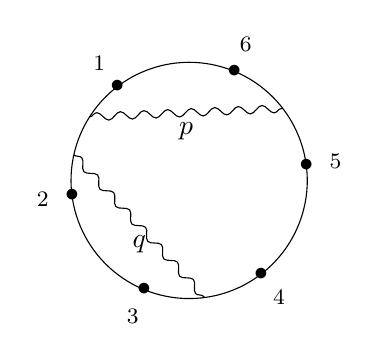
\begin{tikzpicture}[rotate=67.5,baseline=(current bounding box.east)] \begin{scope}
	\drawWLD{6}{1.5}
	\drawnumbers
	\drawlabeledprop{1}{-1}{5}{0}{$p$}
	\drawlabeledprop{1}{1}{3}{0}{$q$}
	\end{scope} \end{tikzpicture} \eas can be written as \bas \VP = \{V_p = \{1, 2, 5,6\} \; ; \; V_1 = \{1, 2, 3,4 \} \} \;.\eas with a matrix \bas M_{\VP} = \begin{bmatrix} x_{p,1} &  x_{p,2} & 0 & 0 &x_{p,5} &x_{p,6} \\x_{q,1} &  x_{q,2} & x_{q,3} &  x_{q,4}& 0 & 0 \end{bmatrix}\; . \eas The Grassmann Necklace of $\Sigma(\VP)$ is $GN(W) = \{ \{12\},\{23\}, \{35\}, \{45\}, \{51\}, \{61\} \}$. From \cite{casestudy}, we see that $\Sigma(\VP)$ shares a boundary with the positroid cells corresponding to \bas M_{\cV_1} = \begin{bmatrix} x_{1,1} &  x_{1,2} & 0 & 0 & 0 &x_{1,6} \\0 &  x_{2,2} & x_{2,3} &  x_{2,4}& x_{2,5} & x_{2,6} \end{bmatrix}  \quad \textrm{and} \quad M_{\cV_2} = \begin{bmatrix} x_{1,1} &  x_{1,2} & x_{1,3} & 0 & 0 &0 \\0 &  x_{2,2} & x_{2,3} &  x_{2,4}& x_{2,5} & x_{2,6} \end{bmatrix}  \;. \eas In particular, the common boundary is parametrized by the matrix \bas M_{\D\cV} = \begin{bmatrix} x_{1,1} &  x_{1,2} & 0 & 0 & 0 &0 \\0 &  x_{2,2} & x_{2,3} &  x_{2,4}& x_{2,5} & x_{2,6} \end{bmatrix}  \;.\eas This common boundary is 5 dimensional, parameterized for instance by setting one of the stars in each row to be 1 and allowing the other entries to be free. 

From Proposition \ref{res:vanishonbdny}, the vanishing set of $R(\VP)$ is exactly $L(\VP) \setminus \Sigma(\VP)$. We show that there is a codimension 1 boundary of $\Sigma(\VP)$ that does not intersect the vanishing set of $R(\VP)$. 

Let $\Sigma(\cV')$ be the positroid cell defined by the matrix $M_{\cV'}$ as defined in Theorem \ref{res:moving variables}. By construction $\Sigma(\cV')$ lies on the boundary of $\Sigma(\VP)$. We show that $\overline{\Sigma(\cV')}$ does not contain the vanishing loci of any of the factors of $R(\VP)$. The minors $\Delta_{13}$ and $\Delta_{15}$ are both non-vanising on $\Sigma(\cV')$, while $\Delta_{35}$ is uniformly zero. However, on $L(\VP)$, the nonvanishing of the minors $\Delta_{13}$ and $\Delta_{15}$ implies the nonvanishing of the minor $\Delta_{35}$. Since $\Delta_{35}$ vanishes on $\Sigma(\cV')$, $L(\VP)$ does not intersect this boundary and hence $R(\VP)$ does not vanish on $\Sigma(\cV')$.

Note that $W = \{ 3, 4\}$, and $V = \{5, 6\}$ are two cyclic flats of $M_{\VP}$ that satisfy the conditions of the proposition. Then, up to permuations of the rows, there is only one choice for $M_{\cV'}$: \bas M_{\cV'} = \begin{bmatrix} x_{1,1} &  x_{1,2} & 0 & 0 & 0 &0 \\x_{2,1} &  x_{2,2} & x_{2,3} &  x_{2,4}& x_{2,5} & x_{2,6} \end{bmatrix} \;. \eas Note that while this is not the same matrix as $M_{\D\cV}$ these two matrices do represent the same matriod, which can be seen by comparing basis sets. In fact, the matrix $M_{\cV'}$ is a non-minimal representation of the matrix $M_{\D\cV}$.
\end{eg}

\begin{rmk}
As remarked in Example \ref{eg:strangeboundary}, the matrix $M_{\cV'}$ defined above Lemma \ref{res:moving variables} does not have the minimal number of parameters to represent the boundary positroid $\Sigma(\cV')$. In particular, we have that  \bas |\bigcup_{V \in \cV'}V| = 6 \quad \textrm{ while } \max_{V \in  \cV'} (|V|) + |\mathcal{V}| +1 = 5 + 2 +1 = 8 \;.\eas Therefore, setting $\cV' = \mathcal{T}$, we see that the third equivalence of Theorem \ref{res:minimalrep} doesn't hold, and thus $M_{\cV'}$ is not a minimal representation. In fact, there is a $GL(k)$ transformation taking $M_{\cV'}$ to $M_{\D\cV}$: \bas \begin{bmatrix}1 & 0  \\ -\frac{x_{q_1}}{x_{p_1}} & 1 \end{bmatrix}  \begin{bmatrix} x_{p,1}&  x_{p,2} & 0& 0 &0 &0 \\x_{q,1}  &  x_{q,2} & x_{q,3}&  x_{q,4}& x_{q,5} & x_{q,6} \end{bmatrix} =  \begin{bmatrix} x_{p,1}&  x_{p,2} & 0& 0 &0 &0 \\0  &  x_{q,2} -\frac{x_{q_1}x_{p_2}}{x_{p_1}} & x_{q,3}&  x_{q,4}& x_{q,5} & x_{q,6} \end{bmatrix} \eas \end{rmk}



The requirement that $V$ and $W$ are cyclic intervals may seem arbitrary until one considers that all flacets of a matroid are cyclic intervals if and only if the matroid is a positroid, and that all flacets are cyclic intervals. In some moral sense, the algorithm prescribed in Proposition \ref{res:moving variables} aims to combine two flacets into a larger flacets in order to define a new positroid cell. 

In the particular case of Wilson loop diagrams ($W = (\cP, [n])$), recall from Lemma 2.28 of \cite{wilsonloops} that all cyclic flats can be represented as a propagator flat, $F(P)$, and that by Lemma 3.35 of the same, any propagator flat that is a cyclic flat has rank equal to the number of propagators in the set defining it. Therefore, the boundaries of the sort considered in Lemma \ref{res:moving variables} occur when there are two propagators flats $F(P)$ and $F(Q)$ such that \begin{enumerate} \item Neither $P$ nor $Q$ are the full propagators set, $\cP$. \item The sets $F(P)$, $F(Q)$ and $F(P) \cup F(Q)$ form cylic intervals in $[n]$, \item One propagator set is not contained in the other. \end{enumerate} It is easy to check that these conditions are met in the Wilson loop diagram $W$ in Examaple \ref{eg:strangeboundary}.


\subsection{Cancelation of poles on the boundary}

We are now ready to prove the main result of this section: that the singularities of $I(\VP)$ that lie on codimension $1$ boundaries of $\Sigma(\VP)$ all cancel in the tree amplitude. Before we begin, we recall a few facts about the polynomial $R(\VP)$. %As a motivating example, we consider the diagram \ba W =   \begin{tikzpicture}[rotate=67.5,baseline=(current bounding box.east)]
%	\begin{scope}
%	\drawWLD{10}{1.5}
%	\drawnumbers
%	\drawprop{1}{0}{8}{1}
%	\drawprop{3}{0}{8}{0}
%        \drawprop{5}{0}{8}{-1}
%		\end{scope}
%	\end{tikzpicture} \;.\label{eq:relevantexample}\ea %with the associated matrix \bas  M_{\VP}  = \begin{bmatrix}  x_{p,1} & x_{p,2} &0 & 0 & 0 & 0& 0 & x_{p,8} & x_{p,9} & 0 \\ 0 &  0 & x_{r,3} & x_{r,4} & 0  & 0  & 0 & x_{r,8} & x_{r,9} & 0  \\  0 & 0 & 0 &0 &x_{s, 5}  &x_{s,6}& 0  & x_{s,8} & x_{s, 9} & 0 \end{bmatrix} \;.\eas 

We classify effect of setting the factors of $R(\VP)$ to the diagram $W$. By Definition \ref{dfn:I(W)}, the primitive factors of $R(\VP)$ either either have degree one or two, corresponding to $1 \times 1$ or $2 \times 2$ minors of $M_{\VP}$. In particular, if the edge $e$ supports $\{q_1, \ldots, q_s\}$ ordered as in Definitions \ref{dfn:adjascentprops}. The degree one factors of $R(\VP)$ are of the form  $x_{q_1, e+1}$ or $x_{q_s, e}$. Setting these to $0$ corresponds to removing $x_{q_1, e+1}$ from the support of the first propagator ($e+1 \not \in V_{q_1}$, or $x_{q_1, e+1} = 0 $) or removing $x_{q_s, e}$ from the support of the last propagator ($e \not \in V_{q_s}$, or $x_{q_s, e} = 0 $) . Note that there is never any factor of $R(\VP)$ that involves two non-adjascent propagators. %For $W$ as in \eqref{eq:relevantexample}, we depict this diagramatically, for $e = 8$ as 

\begin{comment}
\bas   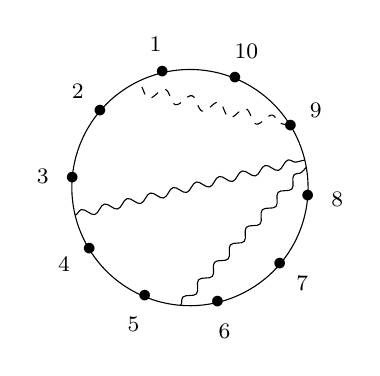
\begin{tikzpicture}[rotate=67.5,baseline=(current bounding box.east)]
	\begin{scope}
	\drawWLD{10}{1.5}
	\drawnumbers
	\boundaryprop{1}{0}{9}{propagator, dashed}
	\drawprop{3}{0}{8}{0}
        \drawprop{5}{0}{8}{-1}
		\end{scope}
	\end{tikzpicture} \text{ or } 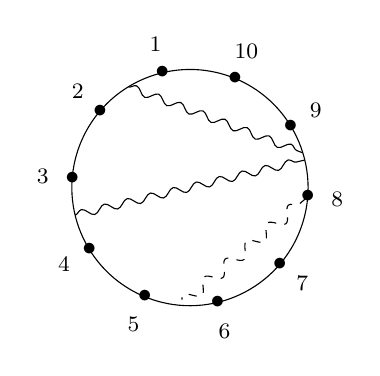
\begin{tikzpicture}[rotate=67.5,baseline=(current bounding box.east)]
	\begin{scope}
	\drawWLD{10}{1.5}
	\drawnumbers
	\drawprop{1}{0}{8}{1}
	\drawprop{3}{0}{8}{0}
        \boundaryprop{5}{0}{8}{propagator, dashed}
		\end{scope}
	\end{tikzpicture} \;.\eas Note that unless there is exactly one propagator adjascent on an edge, there is at most ever one variable corresponding to that edge that is a factor of $R(\VP)$. 

Similarly, the degree two factors corresponds to setting two pairs of variables, ($x_{q_i, e} , x_{q_i e+1}$) and ($x_{q_{i+1}, e} , x_{q_{i+1}, e+1}$), precicely those supporting adjasacent propagators on an edge, as scalar multiples of each other. Diagramatically, we depict this as  we draw this by making two adjascent propagators meet on the common edge. Again, from display \eqref{eq:relevantexample}, with $e = 8$, \bas   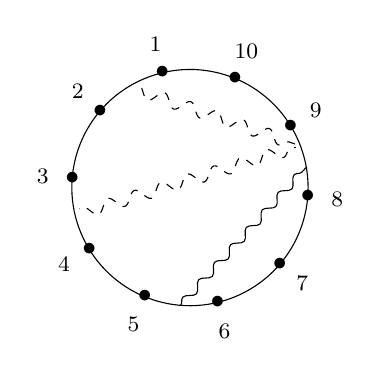
\begin{tikzpicture}[rotate=67.5,baseline=(current bounding box.east)]
	\begin{scope}
	\drawWLD{10}{1.5}
	\drawnumbers
	\modifiedprop{1}{0}{8}{2}{propagator, dashed}
	\modifiedprop{3}{0}{8}{2}{propagator, dashed}
        \drawprop{5}{0}{8}{-1}
		\end{scope}
	\end{tikzpicture} \;.\eas.    \todo{is the diagramatics actualy useful here?}
\end{comment}


\begin{thm} \label{res:deg1polescancel}
All the codimension 1 poles of admissible Wilson loop diagrams cancel.
\end{thm}

\begin{proof}

We first consider all the possible degree 1 factors of $R(\VP)$. Write $W = (\cP, [n])$ with $p= (i,j)  \in \cP$. There are several cases to consider:

\textbf{Case 1:} $  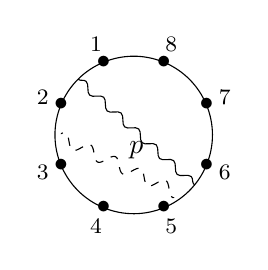
\begin{tikzpicture}[rotate=67.5,baseline=(current bounding box.east)] \begin{scope}
	\drawWLD{8}{1}
	\drawnumbers
	\drawlabeledprop{1}{0}{5}{1}{$p$}
        \modifiedprop{2}{0}{5}{-1}{propagator, dashed}
	\end{scope} \end{tikzpicture} $ Suppose $j > i+2$ (i.e. if $V_p$ does not consist of $4$ cyclically consecutive vertices) and, wihtout loss of generality, assume $x_{p, i}$ is a factor of $R(\VP)$. Then if $q = (i+1, j) \not \in \cP$ the we may define another diagram $W' = ((\cP \setminus p) \cup q, [n])$ that is identical to $W$ except that the propagator $p$ is replaced by $q$. Then $\lim_{x_{p, i} \rightarrow 0} I(\VP) = -\lim_{x_{q, i+2} \rightarrow 0} I(W')$, where the negative sign comes from the evaluation of $\delta^{4k|4k}$ (see Lemma \ref{lem:movingpropnegative}). For more details on the minus signs, see \cite{casestudy, HeslopSteward, correlahedron}. By the arguments of \cite{basisshapeloci}, we see that this parametrizes a co-dimension 1 boundary of $\Sigma(\VP)$ \todo{Cam, what should I cite here?}. It is easy to check that $W'$ satisfies both non-crossing (because $W$ satisfies non-crossing) and the density (because $q \not \in \cP$, and $W$ satisfies density) conditions for admissibility. Therefore $W'$ is admissible. 

\textbf{Case 1a:} $  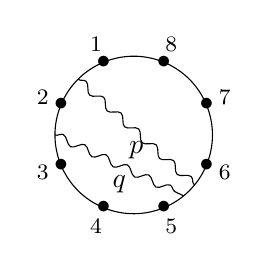
\begin{tikzpicture}[rotate=67.5,baseline=(current bounding box.east)] \begin{scope}
	\drawWLD{8}{1}
	\drawnumbers
	\drawlabeledprop{1}{0}{5}{1}{$p$}
        \drawlabeledprop{2}{0}{5}{-1}{$q$}
	\end{scope} \end{tikzpicture} $  If $q = (i+1, j) \in \cP$, then, in the matrix $\lim_{x_{p, i} \rightarrow 0}M_{\VP}$, the row corresponding to the propagator $p$ now has 3 non-zero entries (corresponding to the columns $\{i+1, j, j+1\}$) and the row corresponding to $q$ has $4$ non-zero entries (corresponding to the columns $\{i+1, i+2, j, j+1\}$). That is, we have $2$ rows with non-zero entries in $4$ columns. Therefore, by Theorem \ref{res:minimalrep}, we see that this locus lies in a boundary of $\Sigma(\VP)$ of codimension of at least 2. Therefore, we do not consider these poles in this argument. 

\textbf{Case 2:}$  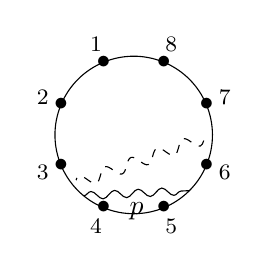
\begin{tikzpicture}[rotate=67.5,baseline=(current bounding box.east)] \begin{scope}
	\drawWLD{8}{1}
	\drawnumbers
	\drawlabeledprop{3}{1}{5}{0}{$p$}
        \modifiedprop{3}{-1}{6}{0}{propagator, dashed}
        \end{scope} \end{tikzpicture} $;  $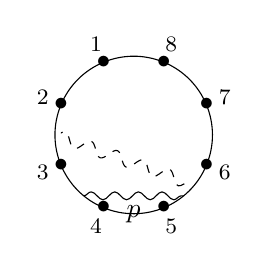
\begin{tikzpicture}[rotate=67.5,baseline=(current bounding box.east)] \begin{scope}
	\drawWLD{8}{1}
	\drawnumbers
	\drawlabeledprop{3}{1}{5}{-1}{$p$}
        \modifiedprop{2}{0}{5}{1}{propagator, dashed}
        \end{scope} \end{tikzpicture} $; $  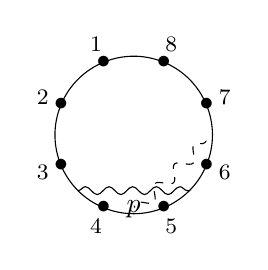
\begin{tikzpicture}[rotate=67.5,baseline=(current bounding box.east)] \begin{scope}
	\drawWLD{8}{1}
	\drawnumbers
	\drawlabeledprop{3}{0}{5}{0}{$p$}
        \modifiedprop{4}{0}{6}{0}{propagator, dashed}
        \end{scope} \end{tikzpicture} $ Next, consider the degree one factors of $R(\VP)$ contributed by propagators of the form $p = (i, i+2)$. If $x_{p, i+1}$ or $x_{p, i+2}$ is a factor of $R(\VP)$, then consider the propatator $q = (i-1, i+2)$ or $q = (i, i+3)$ respectively. If $q \not \in \cP$, then the diagram $W' = ((\cP \setminus p)\cup q, [n])$ is admissible, and the argument proceeds as Case 1. If $q \in \cP$, then the argument proceeds as in Case 1a.  If $x_{p, i}$ or $x_{p, i+3}$ is a factor of $R(\VP)$, consider $q = (i+1, i+3)$ and $q = (i-1, i+1)$ respectively. By the non-crossing condition, $p$ and $q$ cannot simultaneously exist in $W$. If $W$ does not contain another propagator of the form $(i+2, k)$ or $(i, k)$ respectively, we may define an admissible diagram $W' = ((\cP \setminus p)\cup q, [n])$ (otherwise, $q$ would cross the existing propagator $(i+2, k)$ or $(i, k)$).  In this case, $\lim_{x_{p, i} \rightarrow 0} I(\VP) = -\lim_{x_{q, i+4} \rightarrow 0} I(W')$ where the negative sign again comes from Lemma \ref{lem:movingpropnegative}.

\textbf{Case 2a:}$  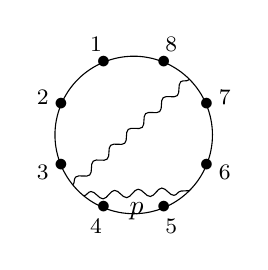
\begin{tikzpicture}[rotate=67.5,baseline=(current bounding box.east)] \begin{scope}
	\drawWLD{8}{1}
	\drawnumbers
	\drawlabeledprop{3}{1}{5}{0}{$p$}
        \drawlabeledprop{3}{-1}{7}{0}{}
        \end{scope} \end{tikzpicture} $ ; $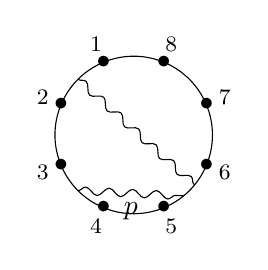
\begin{tikzpicture}[rotate=67.5,baseline=(current bounding box.east)] \begin{scope}
	\drawWLD{8}{1}
	\drawnumbers
	\drawlabeledprop{3}{0}{5}{-1}{$p$}
        \drawlabeledprop{1}{0}{5}{1}{}
        \end{scope} \end{tikzpicture} $ When $x_{p, i}$ (resp. $x_{p, i+3}$) is a factor of $R(\VP)$ and there exists a propagator $(i+2, k)$ (resp. $(i, k)$) in $W$, the singularity formed by sending $x_{p, i}$ (resp. $x_{p, i+3}$) to zero cancels with a pole coming from degree 2 factors contributed by other diagrams. Therefore, we return to this during the discussion of $2 \times 2$ minors. 

\textbf{Case 3:}  $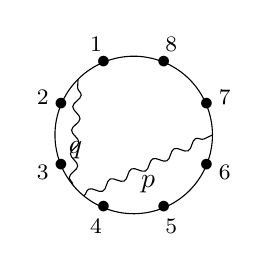
\begin{tikzpicture}[rotate=67.5,baseline=(current bounding box.east)] \begin{scope}
	\drawWLD{8}{1}
	\drawnumbers
	\drawlabeledprop{3}{1}{6}{0}{$p$}
        \drawlabeledprop{3}{-1}{9}{0}{$q$}
        \end{scope} \end{tikzpicture} $ Next, we consider the degree 2 factors of $R(\VP)$. If such a factor to exists, there must be two propagators $p = (i, j)$ and $q = (i, k)$ adjacent on the edge $i$. Suppose $k > j+1$, that is, the other endpoints of $p$ and $q$ are not on adjascent edges. If $r = (j,k) \not \in \cP$, consider two other diagrams formed by replacing the propagator $p$ and $q$ by r: $W' = (\cP' = (\cP \setminus p) \cup r, [n])$ and $W'' = (\cP'' = (\cP \setminus q) \cup r, [n])$. Since $k> j+1$ and $r \not \in \cP$, both $W'$ and $W''$ both satisfy density. Furthermore, since $W$ is admssible, and $p$ and $q$ are adjascent on the edge $i$, there does not exist a propagator $(i, m)$ with $j < m <k$, that is, that has one endpoint on the $i^{th}$ edge, and the other between the other endpoints of $p$ and $q$. Therefore, $W'$ and $W''$ satisfy the non-crossing condition. Thus, $W'$ and $W''$ are both admissible. Note that the diagrams $W$, $W'$ and $W''$ are in the configuration layed out in display \eqref{eq:wideV}. By Theorem \ref{res:Rado}, we see that the reparametrization performed in Lemma \ref{res:Vdiagcancel} means that $\lim_{(x_{p,i}x_{q,i+1} -x_{p,i+1}x_{q,i})\rightarrow 0} M_{\VP}$  parameterized a codimension 1 subspace of $\overline{\Sigma(\VP)}$. By Proposition \ref{res:vanishonbdny}, this is lies in a codimension 1 boundary of $\Sigma(\VP)$. Accoring to Lemma \ref{res:Vdiagcancel}, after appropriate changes of parametrizations, one may write \bas \lim_{(x_{r,k}x_{q,k+1} -x_{r,k+1}x_{q,k})\rightarrow 0}I(\VP') +  \lim_{(x_{p,i}x_{q,i+1} -x_{p,i+1}x_{q,i})\rightarrow 0} I(\VP) + \lim_{(x_{p,j}x_{r,j+1} -x_{p,j+1}x_{r,j})\rightarrow 0}I(\VP'') = 0 \; .\eas 
\begin{comment}
That is, the limits represented by the following diagrams, paramterize the same codimension 1 subspace in the intersection $\Sigma(\VP) \cap \Sigma(\VP') \cap \Sigma(\VP'')$.    \bas 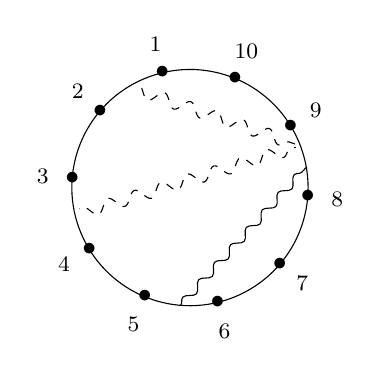
\begin{tikzpicture}[rotate=67.5,baseline=(current bounding box.east)]
	\begin{scope}
	\drawWLD{10}{1.5}
	\drawnumbers
	\modifiedprop{1}{0}{8}{2}{propagator, dashed}
	\modifiedprop{3}{0}{8}{2}{propagator, dashed}
        \drawprop{5}{0}{8}{-1}
		\end{scope}
	\end{tikzpicture} \leftrightarrow 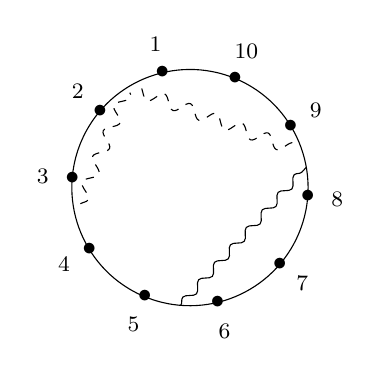
\begin{tikzpicture}[rotate=67.5,baseline=(current bounding box.east)]
	\begin{scope}
	\drawWLD{10}{1.5}
	\drawnumbers
	\modifiedprop{1}{0}{8}{1}{propagator, dashed}
	\modifiedprop{1}{0}{3}{0}{propagator, dashed}
        \drawprop{5}{0}{8}{-1}
		\end{scope}
	\end{tikzpicture} \leftrightarrow 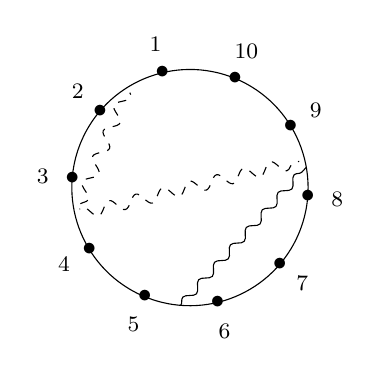
\begin{tikzpicture}[rotate=67.5,baseline=(current bounding box.east)]
	\begin{scope}
	\drawWLD{10}{1.5}
	\drawnumbers
	\modifiedprop{1}{0}{3}{0}{propagator, dashed}
	\modifiedprop{3}{0}{8}{0}{propagator, dashed}
        \drawprop{5}{0}{8}{-1}
		\end{scope}
	\end{tikzpicture}\eas \end{comment}
In otherwords, these three singulariries, which lie on the common codimension 1 boundary positroid of $\Sigma(\VP)$, $\Sigma(\VP')$ and $\Sigma(\VP'')$, cancel in the sum of integrals in the tree level amplitude.

\textbf{Case 3a:} $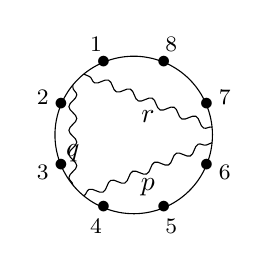
\begin{tikzpicture}[rotate=67.5,baseline=(current bounding box.east)] \begin{scope}
	\drawWLD{8}{1}
	\drawnumbers
	\drawlabeledprop{3}{1}{6}{-1}{$p$}
        \drawlabeledprop{3}{-1}{1}{1}{$q$}
        \drawlabeledprop{6}{1}{1}{-1}{$r$}
        \end{scope} \end{tikzpicture} $ If $k > j+1$ but the propagator $r =  (j,k) \in \cP$, we claim that setting any of the minors $(x_{p,i}x_{q,i+1} -x_{p,i+1}x_{q,i})$, $(x_{p,j}x_{r,j+1} -x_{p,j+1}x_{r,j})$ or $(x_{r,k}x_{q,k+1} -x_{r,k+1}x_{q,k})$ to zero parametrizes a space of codimension greater than 1. As the arguments for all of these are identical, we only show this explicitly for $(x_{p,i}x_{q,i+1} -x_{p,i+1}x_{q,i}) = 0$. Then we may write $x_{q, i} = \lambda x_{p, i}$ and $x_{q, i+1} = \lambda x_{p, i+1}$, with $\lambda$ a real variable. By adding a scalar multiple of the row corresponding to $p$ to the row corresponding to $q$, one may reparametrize $M_{\VP}$ such that the row corresponding to $q$ is supported on the set $V_r =\{j, j+1, k, k+1\}$. Thus, we have 2 propagators supported on $4$ vertices. By Theorem \ref{res:minimalrep}, this is not a minimal representation of $M_{\VP}$. However, in this representation of $M_{\cV}$, the set of variables $\{x_{q, j}, x_{q, j+ 1}, x_{r, j}, x_{r, j+1}\}$ are algebraically independent, and thus the $2 \times 2$ minor they define is diagonalizable by a $GL(k)$ action that acts on the identity on all other rows. Thus after 2 applications of $GL(k)$ transforamations, we have reduced the number of non-zero entries of $M_{\VP}$ by 2, showing that the surface where $(x_{p,i}x_{q,i+1} -x_{p,i+1}x_{q,i}) = 0$ has co-dimension of at least 2 in $\Sigma(\VP)$. \todo{still don't like this argument. Cleaner ideas?}

\textbf{Case 3b:}$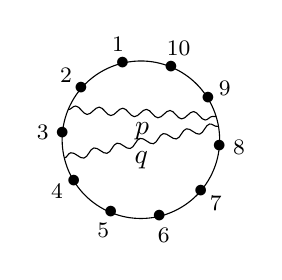
\begin{tikzpicture}[rotate=67.5,baseline=(current bounding box.east)]
	\begin{scope}
	\drawWLD{10}{1}
	\drawnumbers
	\drawlabeledprop{3}{0}{8}{-1}{$q$}
	\drawlabeledprop{2}{0}{8}{1}{$p$}
		\end{scope}
	\end{tikzpicture} $ The final configuration to check is when $p = (i, j)$ and $q = (i, k)$ with $k = j+1$. Consider the diagrams $W' = (\cP' = (\cP \setminus p) \cup r = (j, j+2), [n])$ and $W'' = (\cP'' = (\cP \setminus p) \cup s = (k-2, k), [n])$. Since the edge $r \not \in \cP$ (it would cross $q$ if it were), and $s \not \in \cP$ (it would cross $p$ if it were), we see that $W'$ and $W''$ satisfy both the non-crossing and density conditions, and thus are admissible. Furthermore, $W$, $W'$ and $W''$ are in the configurations layed out in display \eqref{eq:narrowV} and the diagrams $W'$ and $W''$ are in the configuration laid out in Case 2a.

We see from Lemma \ref{res:narrowVcancel} that pole defined by the limit of sending $(x_{p,i}x_{q,i+1} -x_{p,i+1}x_{q,i})$ to $0$ cancels with degree 1 poles in the diagrams in $W'$ and $W''$ under the correct parametrizations: \bas \lim_{(x_{p,i}x_{q,i+1} -x_{p,i+1}x_{q,i}) \rightarrow 0}I(\VP) + \lim_{x_{r, k-2}\rightarrow 0}I(W') + \lim_{x_{s, j+3}\rightarrow 0}I(W'') =0 \;.\eas That is, the limits represented by the following diagrams, paramterize the same codimension 1 subspace in the intersection $\Sigma(\VP) \cap \Sigma(W') \cap \Sigma(W'')$.
\begin{comment}
 \bas 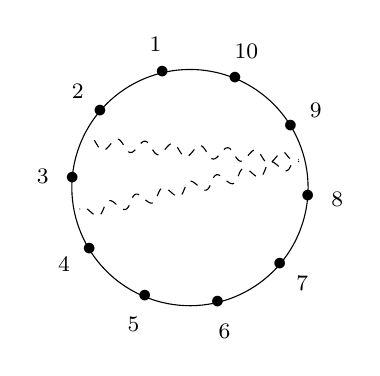
\begin{tikzpicture}[rotate=67.5,baseline=(current bounding box.east)]
	\begin{scope}
	\drawWLD{10}{1.5}
	\drawnumbers
        \modifiedprop{3}{0}{8}{0}{propagator, dashed}
	\modifiedprop{2}{0}{8}{0}{propagator, dashed}
	\end{scope}
	\end{tikzpicture} \leftrightarrow 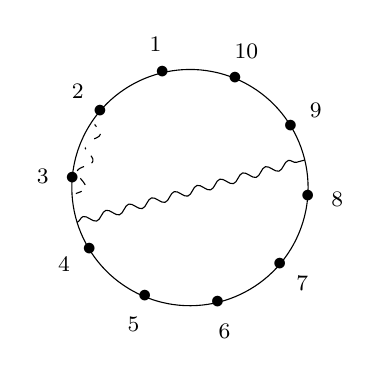
\begin{tikzpicture}[rotate=67.5,baseline=(current bounding box.east)]
	\begin{scope}
	\drawWLD{10}{1.5}
	\drawnumbers
        \drawprop{3}{1}{8}{0}
	\boundaryprop{3}{-1}{2}{propagator, dashed}
	\end{scope}
	\end{tikzpicture} \leftrightarrow 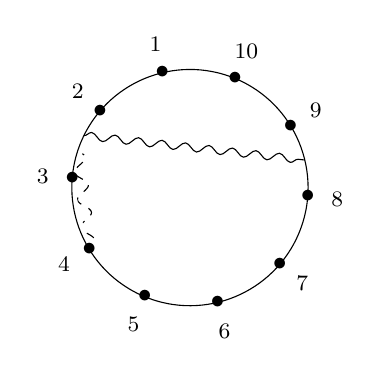
\begin{tikzpicture}[rotate=67.5,baseline=(current bounding box.east)]
	\begin{scope}
	\drawWLD{10}{1.5}
	\drawnumbers
        \drawprop{2}{-1}{8}{0}
	\boundaryprop{2}{1}{4}{propagator, dashed}
	\end{scope}
	\end{tikzpicture}\eas
\end{comment}

\end{proof}


\begin{rmk}
We remark that this cancelation is exact only in the space parametrized by matrices of the form $M(\VP)$, as a subspace of $\Gr(k,n)$ and not in the space parametrized by matrices of the form $M(\YP)$, as a subspace of $\Grall(k,n+1)$. In \cite{HeslopStewart,non-orientability}, the authors explicitly show that cancelations of this form do not hold in the larger space because of orientation issues.
\end{rmk}

\begin{appendices} 
\section{Graveyard of Technical Lemmas \ref{sec:appendix}} 
In this section, we present some calculations to aid in the understanding of the cancelation of spurious poles. Many of the results here can be found in \cite{casestudy, correlahedron, HeslopStewart}. However, they are presented here for completeness.

Recall from Definition \ref{dfn:I(W)} that \bas \cI(\VP) (\cZ_*)  = \int_{(\RP^4)^k} \frac{\prod_{p \in \cP} \prod_{v \in V_p} dx_{p, v}}{R(\VP)} \delta^{4k|4k}(M_{\YP} \cdot \cZ_*) \eas where, for $X$ a $k \times n+4$ matrix, \bas \delta^{4k|4k}(X) = \prod_{b =1}^k (X_{b, 4+b})^4\delta^4((X_{b,1},X_{b,2},X_{b,3},X_{b,4}))  \;.\eas Write $\cZ_*^i$ to indicate the $i^{th}$ column of $\cZ_*$ and $\cZ_*^\mu$ to indicate the matrix formed by taking the first 4 columns of $\cZ_*$. Then evaluating the integral $I(\VP)$ corresponds to localizing the expression \bas \frac{\prod_{b = 1}^k (Y_b \cdot \cZ_*^b)^4}{R(\VP)}\eas at the solution to $M_{\YP} \cdot \cZ_*^\mu = 0$. Writing the propagator $p = (i, j)$ with $i <j$,  Cramer's rule implies that this localization evaluates to \ba x_{p, 0} &= \det(Z_i^\mu, Z_{i+1}^\mu, Z_{j}^\mu, Z_{j+1}^\mu ) \\ x_{p, i} = \det(Z_0^\mu, Z_{i+1}^\mu, Z_{j}^\mu, Z_{j+1}^\mu ) \; &; \; x_{p, i+1} = \det( Z_{i}^\mu, Z_0^\mu, Z_{j}^\mu, Z_{j+1}^\mu ) \; \text{ etc.} \label{eq:matrixvalues}\ea That is, the entry $x_{p, m}$ evaluates to the minor of $\cZ_*^\mu$ indicated by the rows in $V_p$, with the $m^{th}$ row replaced by $Z_0^\mu$.

\begin{lem} \label{lem:movingpropnegative}
For two propagators $p = (i, j)$ and $q = (i, j+1)$, after localization $x_{p, j} = -x_{q, j+2}$
\end{lem} 

\begin{proof}
By the above arguments, note that $x_{p, j} = \det(Z_i^\mu, Z_{i+1}^\mu, Z_{0}^\mu, Z_{j+1}^\mu )$ while $x_{q, j+2} = \det(Z_i^\mu, Z_{i+1}^\mu, Z_{j+1}^\mu , Z_{0}^\mu )$. Thus these two values are negatives.
\end{proof}

Sometimes, as in Theorem \ref{res:polesonboundaries} and Theorem \ref{res:deg1polescancel}, it is necessary to perform changes of variables in order to perform the cancellation of variables. For ease of calculation, we introduce a simplifying change of variables:
\begin{lem}\label{lem:simplifyR(W)}
Consider two propagators $p = (i, j)$ and $q = (i, k)$ that are adjacent on the $i^{th}$ edge of a Wilon loop diagram $(\cP, [n])$, with $p$ appearing closer to the vertex $i$ and $q$ closer to the vertex $i+1$. There is a reparametrization of the matrix $M_{\VP}$ under which one can replace the factor $x_{p, i}(x_{p, i}x_{q, i+1} - x_{p, i+1}x_{q, i})x_{q, i+1}$ in $R(\VP)$ with the product of 4 terms: $xyzw$.
\end{lem}

\begin{proof}
We restrict our attention to the relavant $2 \times 2$ minor of $M_{\YP}$, $ \begin{bmatrix} x_{p, i} & x_{p, i+1} \\ x_{q, i} & x_{q, i+1} \end{bmatrix} $,  which we can reparametrize as $ \begin{bmatrix} x & y \\ xz & zy + w \end{bmatrix} $. Then we have that \bas x_{p, i} = x \quad ; \quad  x_{p, i+1} = y \quad ; \quad x_{q, i} = xz\quad  ;\quad x_{q, i+1}  = zy + w \; . \eas Furthermore, \bas dx_{p, i} = dx  \quad ; \quad  d x_{p, i+1} = dy \quad ; \quad dx_{q, i} = x dz + z dx \quad ; \quad d x_{q, i+1} = ydz + z dy + dw \;.\eas Therefore, under these changes of variables, we see that \bas \frac{dx_{p, i}\;dx_{p, i+1}\;dx_{q, i}\;dx_{q, i+1}}{x_{p, i+1}(x_{p, i}x_{q, i+1} - x_{q, i}x_{p, i+1} ) x_{q, i}}  = \frac{ dx\;dy\;x dz\; dw}{y (xyz + xw - xyz)xz}\eas which simplifies to the desired result.
\end{proof}

In future, we use whichever parametrization of the $2 \times 2$ minors is convenient. The need for a change of variables comes up in two cases. The first case involves the cancelation of the $2 \times 2$ minors in following three propagator confgurations (see Case 3 for Theorem \ref{res:deg1polescancel}): \bml  \textrm{Config 1} = 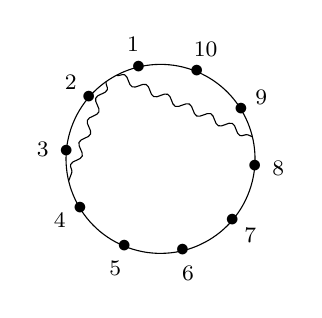
\begin{tikzpicture}[rotate=67.5,baseline=(current bounding box.east)]
	\begin{scope}
	\drawWLD{10}{1.2}
	\drawnumbers
	\drawprop{1}{-1}{8}{0}
	\drawprop{1}{1}{3}{0}
		\end{scope}
	\end{tikzpicture} \quad ; \quad \textrm{Config 2} = 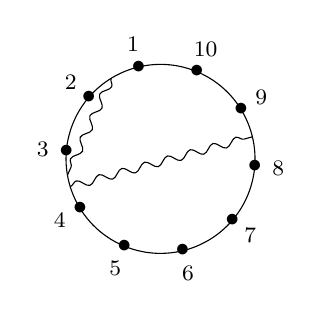
\begin{tikzpicture}[rotate=67.5,baseline=(current bounding box.east)]
	\begin{scope}
	\drawWLD{10}{1.2}
	\drawnumbers
	\drawprop{1}{0}{3}{-1}
	\drawprop{3}{1}{8}{0}
		\end{scope}
	\end{tikzpicture} \\ \textrm{Config 3} = 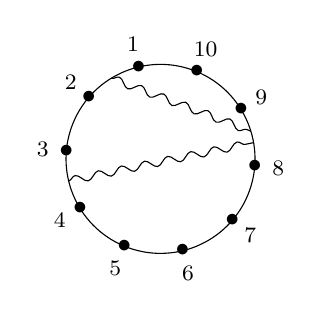
\begin{tikzpicture}[rotate=67.5,baseline=(current bounding box.east)]
	 \begin{scope}
	\drawWLD{10}{1.2}
	\drawnumbers
	\drawprop{1}{0}{8}{1}
	\drawprop{3}{0}{8}{-1}
		\end{scope}
	\end{tikzpicture}  \label{eq:wideV}\eml

\begin{lem}\label{res:Vdiagcancel}
Let $(\cP_1, [n])$, $(\cP_2, [n])$ and $(\cP_3, [n])$ be admissible Wilson loop diagrams that are identical except for the fact that the propagator set $\cP_i$ cotains the pair of adjascent propagators shown in $\textrm{Config i}$ above. Then 
\bas \sum_{i = 1}^3 \lim_{\textrm{degree 2 factor of } R(\cV(\cP_i)) \rightarrow 0} I(\cV(\cP_i)) = 0\;.\eas \end{lem}

This proof is also given in \cite{HeslopStewart, casestudy} but is included here for completeness.
\begin{proof}
Without loss of generality, write $M_{\cY(\cP_i)}$ with the pertinent propagators represented in the first two rows. Then the matrices $M_{\cY(\cP_i)}$ are identical except for the first two rows. Since the propagators are adjacent, by Lemma \ref{lem:simplifyR(W)} we may write the first two rows as \bas M_{\cY(\cP_1)} = \begin{bmatrix}1 & \ldots & a &b &\ldots & 0 & 0 & \ldots & c & d   \ldots\\  1 & \dots &  ae &be + f  & \ldots &g & h & \ldots &0 &0  \ldots   \end{bmatrix}  \\ M_{\cY(\cP_2)} = \begin{bmatrix}1 & \ldots & a' & b' &\ldots & c' & d' & \ldots & 0 & 0   \ldots\\  1 & \dots &  0 & 0  & \ldots &c'e' & d' e' + f' & \ldots &g' &h'  \ldots   \end{bmatrix} \\ M_{\cY(\cP_3)} = \begin{bmatrix}1 & \ldots & 0 &0 &\ldots & a'' & b'' & \ldots & c'' & c''   \ldots\\  1 & \dots &  e'' & f''  & \ldots &0 & 0 & \ldots &c''g'' & d'' g'' + h'' \ldots   \end{bmatrix}\;.\eas We multiply the relavant rows of $M_{\cY(\cP_2)}$ and $M_{\cY(\cP_3)}$ by elements of $GL(2)$, leaving the rest of the rows unchanged. Namely, consider the products: \bas \begin{bmatrix} \frac{- e'}{1-e'} & \frac{1}{1-e'} \\ 1 & 0  \end{bmatrix} M_{\cY(\cP_2)} = \begin{bmatrix}  1 & \dots & \frac{-e' a'}{1- e'}  & \frac{-e' b'}{1- e'}  & \ldots &0 & \frac{ f'}{1-e'} & \ldots &\frac{g'}{1-e'} &\frac{h'}{1-e'}  \ldots  \\ 1 & \ldots & a' & b' &\ldots & c' & d' & \ldots & 0 & 0   \ldots \end{bmatrix}  \\ \begin{bmatrix}  \frac{1}{1-c''} & \frac{-c''}{1-c''}\\ 0  & 1  \end{bmatrix} M_{\cY(\cP_3)} = \begin{bmatrix}1 & \ldots & \frac{-e''c''}{1-c''} &\frac{-f''c''}{1-c''} &\ldots & a'' & b'' & \ldots & 0 & \frac{d''}{1-c''}   \ldots\\  1 & \dots &  e'' & f''  & \ldots &\frac{a''}{1-c''} & \frac{b''}{1-c''} & \ldots &g'' & h'' \ldots   \end{bmatrix}\;.\eas
From this, we see that, in the limit $f \rightarrow 0$ and $M_{\cY(\cP_1)}$ and $f' \rightarrow 0$ for $\begin{bmatrix} \frac{- e'}{1-e'} & \frac{1}{1-e'} \\ 1 & 0  \end{bmatrix} M_{\cY(\cP_2)}$, we have the change of variables \bmls a = \frac{-e'a'}{1-e'} \quad ; \quad b = \frac{-e'b'}{1-e'} \quad ; \quad c = \frac{g'}{1-e'} \quad ; \quad d = \frac{d}{1-e'}  \quad ; \\ \quad e = \frac{1-e'}{e'}\quad ; \quad f = 0 \quad ; \quad g = c' \quad ; \quad h = d'\;.\emls Inverting and performing the change of variables, we see that $\lim_{f' \rightarrow 0} I(\cV(\cP_2)) = \lim_{f \rightarrow 0} \frac{-1}{1-e} I(\cV(\cP_1))$. A similar calculation shows that $\lim_{d'' \rightarrow 0} I(\cV(\cP_3)) = \lim_{f \rightarrow 0} \frac{e}{1-e} I(\cV(\cP_1))$. Thus, in the appropriate limit, \bas \lim_{f \rightarrow 0} I(\cV(\cP_1)) + \lim_{f' \rightarrow 0} I(\cV(\cP_2)) + \lim_{d'' \rightarrow 0} I(\cV(\cP_3)) = 0\;.\eas  \end{proof} \todo{actually check these calculations, minus signs, etc.}

The last case to consider consists of understanding the poles shared between the diagrams with the following configureations: \bml \textrm{Config 4} = 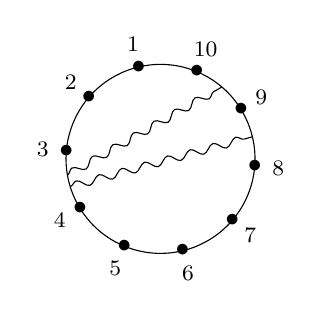
\begin{tikzpicture}[rotate=67.5,baseline=(current bounding box.east)]
	 \begin{scope}
	\drawWLD{10}{1.2}
	\drawnumbers
	\drawprop{3}{-1}{9}{0}
	\drawprop{3}{1}{8}{0}
		\end{scope}
	\end{tikzpicture} \quad ; \quad \textrm{Config 5} = 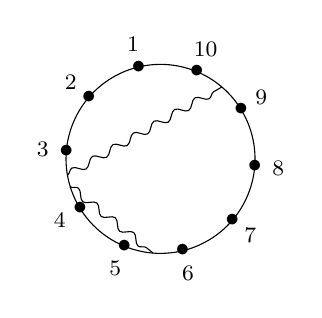
\begin{tikzpicture}[rotate=67.5,baseline=(current bounding box.east)]
	\begin{scope}
	\drawWLD{10}{1.2}
	\drawnumbers
	\drawprop{3}{-1}{9}{0}
	\drawprop{3}{1}{5}{0}
		\end{scope}
	\end{tikzpicture} \\ \textrm{Config 6} = 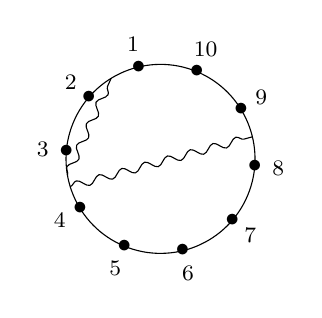
\begin{tikzpicture}[rotate=67.5,baseline=(current bounding box.east)]
	\begin{scope}
	\drawWLD{10}{1.2}
	\drawnumbers
	\drawprop{3}{-1}{1}{0}
	\drawprop{3}{1}{8}{0}
		\end{scope}
	\end{tikzpicture} \label{eq:narrowV}\eml

\begin{lem}\label{res:narrowVcancel}
Let $(\cP_4, [n])$, $(\cP_5, [n])$ and $(\cP_6, [n])$ be admissible Wilson loop diagrams that are identical except for the fact that the propagator set $\cP_i$ cotains the pair of adjascent propagators shown in $\textrm{Config i}$ above. Let $p = (i, j)$ and $q = (i, k)$ with $k = j+1$. Then \bas \lim_{(x_{p,i}x_{q, i+1} - x_{p, i+1}, x_{q, i}) \rightarrow 0} I(\cV(\cP_4)) + \lim_{x_{r, j+3} \rightarrow 0}I(\cV(\cP_5)) + \lim_{x_{r, k-2} \rightarrow 0}I(\cV(\cP_6)) = 0\;.\eas \end{lem}
\begin{proof}
This proof follows similarly to the above. Write \bas M_{\cY(\cP_4)} = \begin{bmatrix}1 & \ldots & a &b &\ldots & c & d & 0 & \ldots \\  1 & \dots &  ae &be + f  & \ldots &0 & g & h & \ldots    \end{bmatrix}  \\ M_{\cY(\cP_5)} = \begin{bmatrix}1 & \ldots & a' &b' &\ldots & c' & d' & 0 & 0& \ldots \\  1 & \dots &  0&0  & \ldots &c'e' & d'e' +f' & g' & h' & \ldots    \end{bmatrix} \\ M_{\cY(\cP_6)} = \begin{bmatrix}1 & \ldots & 0 &0 &\ldots & a'' & b'' & c''g'' & h'' c'' + d'' & \ldots \\  1 & \dots &  e'' & f''  & \ldots &0&0 & g'' & h'' & \ldots    \end{bmatrix} \;. \eas We consider the change of variables defined by the product \bas \begin{bmatrix}1 & 0 \\ \frac{-e'}{1-e'} & \frac{1}{1-e'} \end{bmatrix} M_{\cY(\cP_5)}  \quad \textrm{ and } \quad \begin{bmatrix}\frac{1}{1-c''} & \frac{-c''}{1-c''} \\ 0 & 1 \end{bmatrix} M_{\cY(\cP_6)} \;.\eas Then the same types of calculations as in Lemma \ref{res:Vdiagcancel} shows that $ \lim_{x_{r, k-2} \rightarrow 0}I(\cV(\cP_6))  =  \lim_{f \rightarrow 0} \frac{-1}{1-e} I(M_{\cV(\cP_4)}) $ and $\lim_{x_{r, k-2} \rightarrow 0}I(\cV(\cP_5))  =  \lim_{f \rightarrow 0} \frac{e}{1-e} I(\cV(\cP_4)) $, proving the result.
\end{proof}


%Let $\mathcal{P} = \{P_1, P_2, \dots, P_k\}$ be a collection of subsets of $\{1,2,\dots,n\}$. Let $\mathbf{x}=\{x_{i,j}\}$ be algebraically independent invertible variables. Define $M_{\mathcal{P}}(\mathbf{x})$ to be the $n \times k$ matrix having $x_{i,j}$ as its $i,j$ entry if $j \in P_i$ and $0$ otherwise.

Finally, we show that the limits defined in Lemma \ref{res:Vdiagcancel} and Lemma \ref{res:narrowVcancel} do infact give rise to codimension 1 boundaries of $\Sigma(\VP)$. To do this, we define a more general result. In Theorem \ref{res:Rado}, we show that, if $M'$ is a variable valued matrix formed by applying an invertible change of variables to a matrix $M_\cV$, then sending $k$ variables to $0$ in $M'$ drops the dimension of the parametrized space $L(M')$ if and only if no row of $M'$ is contained in the span of any other subset of rows of $M'$.

The results is a generalization of the equivalence of 1 and 3 in Theorem \ref{res:minimalrep}. Condition 3 from Theorem \ref{res:minimalrep} is analogous to the inequality from Hall's Matching Theorem. However, 
the matrices in Theorem \ref{res:minimalrep} have the restriction that entries are either zero or totally independent. Theorem \ref{res:Rado} below, relaxes this condition, allowing one to view each independent non-zero entry as a function of several variables, and setting one of these component variables to $0$, as in Lemma \ref{res:Vdiagcancel} and Lemma \ref{res:narrowVcancel}. 

We begin with a few definitions. 

\begin{dfn}
For an $k \times n$ variable valued matrix $M$ and a set $I \subseteq [k]$, define $M_I$ to be the matrix formed by restricting $M$ to the rows $I$, and let $\mathrm{span}(M_I)$ be the subset of $\mathbb{R}^n$ obtained by evaluating linear combinations of the rows $M$ indexed by $I$ at real parameters. Let $\mathrm{span}(M_{\emptyset})$ be the origin in $\mathbb{R}^n$.
\end{dfn}

Note that these matrices are different from the variable valued matrices defined by $M_{\cV}$ above. We relax the requirement that each entry of the matrix be algebraically independent of all the others. Furthermore, while the entries of $M_I$ are functions of independent variables, the entries themselves may be related by algebraic functions.

\begin{dfn}
Let $L(M_I)$ be the locus of the variable valued matrix $M_I$ in $\Grall(|I|, n)$, as given by the map in \eqref{eq:maps}.
\end{dfn}

\begin{eg}
Let
%
\begin{displaymath}
M =
\begin{bmatrix}x_1 & x_2 & 0 & 0 \\
0 & 0 & x_1 & 0 \\
0 & 0 & x_2 & x_1 \end{bmatrix}.
\end{displaymath}
\noindent
Then, $\mathrm{span}(M_{12})$ consists of all points in $\mathbb{R}^4$ whose last coordinate is zero. On the other hand, $\mathrm{span}(M_{13})$ consists of points of the form $(a,b,\frac{bc}{a},c)$ for some \hlfix{$a,b,c \in \mathbb{R} \setminus \{0\}$}{$b, c \in \R$; $a \in \R^\times$?} together with points of the form $(0,b,c,0)$. Finally, $\mathrm{span}(M_{123})$ is all of $\mathbb{R}^4$.
\end{eg}

\begin{thm}\label{res:Rado}
Let $\cV$ be a collection of subsets, and let $\mathbf{x} = x_{i,j}$ and $\mathbf{y} = y_{i,j}(\mathbf{x})$ be two sets of algebraically independent invertible variable which are related by an invertible change of variables. Let $M_{\cV}(\mathbf{x})$ and $M_{\cV}(\mathbf{y})$ be the variable valued matrices associated to $\cV$ in the variables $\mathbf{x}$ and $\mathbf{y}$. Let $S \subset \mathbf{x}$ be a subset of the variables $\bf{x}$, and write $M' = M_{\mathcal{P}}(\mathbf{y})|_{x_{i,j} = 0; x_{i,j} \in S}$.  Denote by $d = |\mathbf{x}| - |S|$ the number of variables in $\mathbf{x}$ remaining. %Let $L(M')$ be the subset of $\Gr(k,n)$ consisting of row spaces of matrices obtained by evaluating the remaining $x_{i,j}$ in $M'$ at real parameters. 
The following are equivalent: 
\begin{itemize}
\item[(i)] For all $I \subsetneq [k]$ and all $j \in I^c$, $\mathrm{span}(M_I) \subsetneq \mathrm{span}(M_{I \cup j})$. That is, adding a row to $\mathrm{span}(M_I)$ always increases the size of the span.
\item[(ii)] $\mathrm{dim}(L(M')) = d-k$.
\end{itemize}
\end{thm}

\begin{rmk}
% This relaxation on the matrix side of the theorem is mirrored by a relaxation of the inequality from Hall's Matching Theorem. 
Namely, Rado's Theorem, which says that if $S_1, \dots, S_k \subseteq \mathbb{R}^{n}$, then it is possible to select linearly independent vectors $s_1 \in S_1, \dots, s_k \in S_k$ if and only if for all $I \subseteq [k]$,
%
\begin{displaymath}
\mathrm{dim}\left(\mathrm{span}\left( \bigcup_{i \in I} S_i \right) \right) \geq |I|.
\end{displaymath}
%
\noindent
Condition (ii) from Theorem \ref{res:Rado} relaxes this condition from Rado's theorem, saying not only does any subset of vectors have the correct dimension, but adding a new vector always increases the dimension.
\end{rmk}

\begin{proof}\sanote{Cam: changed all $\Gr$ to $\Grall$ in this theorem. Correct?}
We show that (ii) implies (i) via induction on $k$, the number of rows of $M_\cV(\bf{x})$. When $k = 1$, $L(M')$ is a parameterized subset of projective space. Since the transformation from the $\mathbf{x}$ to the $\mathbf{y}$ variables are invertible, $M' = M_{\cP}(\mathbf{y})|_{x_{i,j} = 0; x_{i,j} \in S}$ and $M_{\cP}(\mathbf{x})|_{x_{i,j} = 0; x_{i,j} \in S}$ have the same dimesion in $\R^n$. One obtains the corresponding locus in projective space by scaling by a constant, so the dimensions in projective space remain the same. 

For larger $k$, it is not sufficient to use the invertibility of the change of variables as an argument that the dimension does not change. While this holds on the level of matrices, it may not hold after quotienting by $GL(k)$ in order to find the locus $L(M')$.

Suppose that the result holds for $k = l-1$. Let $M'$ be an $l \times n$ matrix such that $\mathrm{span}(M'_{\{1,\dots,l\}}) = \mathrm{span}(M'_{1,\dots,l-1})$, but that $\mathrm{span}(M'_I) \neq \mathrm{span}(M'_{I \cup j})$ for $j \notin I$ whenever \hlfix{$|I| < l$}{$l-1$? see red}. {\color{red}That is, condition (i) fails to hold only for the sets $|I| = l-1$.} \st{For any subset $I \subset [k]$, let $d_I$ be the number of parameters in the $\mathbf{x}$ variables appearing in the rows of $M'$ indexed by $I$.}\sanote{nix. Not used. $d_l$ means something else below}

\hlfix{Note that $L(M')$ is spanned by an element $r \in  \mathrm{span}(M'_{l})$, plus a $l-1$ plane in $L(M'_{1,\dots,l-1}) \cap \Grall(\mathbb{R}^n \perp r, k-1)$}{why?}. \todo{can we talk about planes in $\Grall$?}\todo{We talk about a span of a vector in $\R^n$ and a subspace of $\Grall$. That can't be right?!} Since condition (i) does not hold for $I = \{1,\dots,l-1\}$, $r \in \mathrm{span}(M'_{1, \dots, l-1})$,
% 

\begin{displaymath}
\dim(L(M'_{1,\dots,l-1}) \cap \Grall(k-1, \mathbb{R}^n \perp r)) < \dim(L(M'_{1,\dots,l-1})). 
\end{displaymath}\todo{why?}
%
\noindent
So,
%
\begin{displaymath}
\dim(L(M')) \leq \dim(L(M'_{l})) + (\dim(L(M'_{1,\dots,l-1})) - 1) = d -k - 1,
\end{displaymath}\todo{why?}
%
\noindent
and thus (ii) implies (i) when $k = l$.

Next, we show that (i) implies (ii). When $k = 1$, $L(M')$ is again a parameterized subset of projective space, and the argument holds similarly to the case for $k=1$ in the other direction of this proof. 

Suppose the result holds for $k = l-1$ and let $M'$ be an $l \times n$ matrix such that $\mathrm{span}(M'_{1,\dots,l}) \neq \mathrm{span}(M'_{1,\dots,l-1})$. Let $d_l$ be the number of parameters appearing in row $l$ of $M'$ which do not appear in rows $1, \dots, l-1$. Note that $L(M'_l)$ is $d_l -1$ dimensional by similar arguments as the base case.

Then, for generic point $r \in \mathrm{span}(M'_{l})$ that comes from evaluating the last row of $M'$, note that $r \notin \mathrm{span}(M'_{1,\dots,l-1})$. So,
%
\begin{displaymath}
\dim(L(M'_{1,\dots,l-1})) \cap \Grall(k-1, \mathbb{R}^n \perp r)) = \dim(L(M'_{1,\dots,l-1})) = d - d_l -(k-1)\;.
\end{displaymath}
%
\noindent
Thus,
%
\begin{displaymath}
\dim(L(M'_{1,\dots,l})) = (d_l - 1) + \dim(L(M'_{1,\dots,l-1})) = d-k.
\qedhere
\end{displaymath}
\end{proof}

Given Theorem \ref{res:Rado}, we see that the boundaries defined in Lemma \ref{res:Vdiagcancel} and Lemma \ref{res:narrowVcancel} do infact give rise to codimension 1 boundaries of $\Sigma(\VP)$.

\begin{cor}
After the reparametrization define in Lemma \ref{lem:simplifyR(W)}, setting $y$, $z$ or $w$ to zero reduces the dimension by $1$.
\end{cor}
\begin{proof}
{\color{red} Not sure how to prove this, or what is going on here? For instance, if we set $x \rightarrow 0$ in Lemma \ref{lem:simplifyR(W)}, we set two of the original variables to 0, and thus drop the dimension by 2. For all others, setting a variable to 0 reduces the dimension by 1 }
\end{proof}

\end{appendices}








\end{document}
